% =====================================================================
% StaticKD -- single-file manuscript (IEEEtran journal layout)
% Built by scripts/build_paper.py from src/paper/ and the notebook outputs; numbers are literal.
% results/final/paper_number_map.json lists every number; scripts/check_paper.py reports changes.
% Compile: pdflatex main && bibtex main && pdflatex main && pdflatex main
% =====================================================================
\documentclass[journal]{IEEEtran}

\usepackage[T1]{fontenc}
\usepackage[utf8]{inputenc}
\usepackage[nocompress]{cite}
\usepackage{amsmath,amssymb}
\usepackage{graphicx}
\usepackage{booktabs}
\usepackage{multirow}
\usepackage{array}
\usepackage{xcolor}
\usepackage[hyphens]{url}
\usepackage{algorithm}
\usepackage{algpseudocode}
\usepackage{tikz}
\usetikzlibrary{positioning,arrows.meta,fit,calc}

\DeclareRobustCommand{\todo}[1]{{\color{red}[TODO: #1]}}

\emergencystretch=1.5em

\begin{document}

\title{StaticKD: Distilling a Multilingual IPTC News Topic Classifier into a Static Token-Logit Table for Lightweight CPU Inference}

\author{Obi~Kastanya and Ananta~Dwi~Prayoga~Alwy%
\thanks{O. Kastanya and A. D. P. Alwy are with the Department of Informatics Engineering, Sepuluh Nopember Institute of Technology, Surabaya, Indonesia (e-mail: 6025252015@student.its.ac.id; 6025252007@student.its.ac.id). Corresponding author: O. Kastanya. This work received no specific funding.}}

\markboth{IEEE Access (draft)}%
{Kastanya and Alwy: StaticKD, Multilingual IPTC News Topic Classification on CPU}

\maketitle

\begin{abstract}
Filtering news by the International Press Telecommunications Council (IPTC) Media Topic taxonomy requires a classifier cheap enough for a multilingual article stream. The available open multilingual IPTC classifier is based on XLM-RoBERTa-large and needs 1,239 to 2,971 milliseconds per article on one processor core. With this classifier as teacher, StaticKD stores 17 scores per vocabulary token, one per top-level IPTC topic. Classifying an article then only requires tokenizing it and averaging its token scores. The student is initialized from multilingual static embeddings (one fixed vector per token) and learns from teacher outputs on 285,999 articles in 69 languages. The evaluation uses a new test set of 12,744 articles in 47 languages. Their topics are assigned by human annotators or newsroom editors and mapped onto IPTC, so no test label comes from a model that reads the article. On this test set, StaticKD reaches a macro-F1 of 0.545, or 91.1\% of the teacher score (0.598). The 34-megabyte model classifies 473 articles per second per core, about 616 times faster than the 8-bit quantized teacher. It is also more accurate than fastText and a linear support vector machine trained on the same teacher labels. Ablations with five seeds show that accuracy comes mainly from multilingual training data and pre-trained cross-lingual embeddings, and that the top teacher label works as well as the full distribution. Fine-tuning the embeddings helps the training languages but hurts unseen languages. StaticKD is weakest on languages absent from both its training data and the teacher's pre-training data.
\end{abstract}

\begin{IEEEkeywords}
Efficient inference, knowledge distillation, multilingual text classification, news topic classification, static embeddings.
\end{IEEEkeywords}

\section{Introduction}
\label{sec:introduction}
\IEEEPARstart{N}{ews} analytics pipelines need topic filtering to prevent irrelevant news from being processed in later stages and adding to the cost. Before being filtered, news articles have to be classified into standardized topic categories, such as those of the Media Topic taxonomy of the International Press Telecommunications Council (IPTC). The IPTC taxonomy divides news topics into 17 top-level categories, which contain many subcategories~\cite{iptc2024mediatopics,kuzman2025llm}.

The first open multilingual IPTC classifier was released by Kuzman and Ljube\v{s}i\'c~\cite{kuzman2025llm}. GPT-4o was used to label articles in four languages, and the labels then served as data for fine-tuning XLM-RoBERTa-large~\cite{conneau2020xlmr}. On a human-annotated test set, the resulting model performs on par with GPT-4o. A follow-up study by the same group concluded that fine-tuned encoders are more practical than large language models (LLMs) for large-scale annotation~\cite{kuzman2025southslavic}. Without a graphics processing unit (GPU), an encoder with 559.9~million parameters remains expensive. The present study targets servers without a GPU, where the classifier shares central processing unit (CPU) cores with the rest of the pipeline. The model needs 2,971~ms per article on one CPU core. Its fastest CPU configuration is an Open Neural Network Exchange (ONNX) export quantized to 8-bit integers (int8), and this configuration still needs 1,239~ms. At such latencies, topic classification alone would occupy 15.1 (ONNX int8) to 34.8 (PyTorch) CPU cores for a stream of one million articles per day (Section~\ref{sec:res-eff}). Neither of the two earlier studies reports this inference cost, although inference accounts for a large share of the computing demand and energy use of machine learning in production. Google, for example, reported that 60\% of its machine learning energy use came from inference~\cite{luccioni2024power}.

Such a pipeline needs a topic classifier that covers many languages and runs in milliseconds per article on an ordinary CPU. The classifier also has to be small and have few dependencies. Small distilled transformers~\cite{sanh2019distilbert,wang2021minilmv2} give a speedup of about one order of magnitude. In the CPU benchmark of this study, MiniLM-L6 runs 21 times faster than the ONNX int8 teacher. Int8 quantization alone gives a 2.3-fold speedup over PyTorch fp32. fastText~\cite{joulin2017bag} is much faster, but it learns its word vectors from scratch and therefore does not support cross-lingual transfer. In this setting, the restriction is serious. The IPTC training labels released with the open classifier cover only four languages~\cite{emmediatopic2025}. Even a corpus labeled automatically by a multilingual teacher cannot contain every language of a news stream. None of the available IPTC classifiers is both multilingual and this cheap.

The StaticKD method proposed in this paper distills~\cite{hinton2015distilling} the XLM-R-large IPTC classifier into a far simpler student. Three properties of the problem make this possible. Unlabeled news in any language can be labeled by a teacher that works across languages, so the training data for the student cost nothing to annotate. Multilingual static embeddings distilled from sentence encoders~\cite{tulkens2024model2vec,wada2025static,chen2024bgem3} give each token one fixed vector and place translation equivalents close to each other. Looking up such a vector costs almost nothing. News topics are also strongly tied to vocabulary, which explains why bag-of-words representations remain competitive for topic classification~\cite{galke2022bow}. The student therefore averages the embeddings of the tokens in an article and then applies one linear layer. Both steps are linear, so the linear layer can be applied once to every embedding before deployment. Applying the layer before deployment is called folding in this paper. Folding turns the model into a table that stores 17 topic scores (logits) per token. Classifying an article then reduces to tokenizing it and averaging the table rows of its tokens. The computation runs in NumPy without a deep learning library. Fig.~\ref{fig:tradeoff} in Section~\ref{sec:res-eff} compares the accuracy and speed of StaticKD with those of the other models.

A multilingual claim also requires a multilingual evaluation with labels that do not come from the teacher. The human-annotated test set of Kuzman and Ljube\v{s}i\'c is not public and covers four languages. SIB-200~\cite{adelani2024sib200} covers 205 languages, but its items are short sentences and its taxonomy is not IPTC. The present study fills this gap by building a unified test set of 12,744 articles in 47 languages. Some of its articles are news pages from 2024 to 2026 whose publishers record the newsroom section of the article in the page metadata (schema.org~\cite{guha2016schema}). The pages are combined with public datasets labeled by human annotators or with publisher categories~\cite{adelani2023masakhanews,petukhova2023mnds,mirashi2023indicnews,hossain2025banglanews}. Each label is an editorial decision of a publisher or an annotator and is then mapped onto the official IPTC taxonomy. The process involves no model that reads the article text.

The study answers four research questions (RQs). RQ1 asks how much of the teacher accuracy StaticKD retains on labels that do not come from the teacher. The comparison uses two baselines of similar cost, namely fastText and a support vector machine (SVM) with term frequency--inverse document frequency (TF-IDF) features. The other models in the comparison are MiniLM-L6 and DistilmBERT, two more expensive small transformers. RQ2 examines which parts of the training recipe matter for this very small student. The tested parts are soft labels, multilingual data, embedding initialization, embedding fine-tuning, token dropout, temperature, and ensembling. For RQ3, the study measures the inference cost of the teacher on CPU and how far StaticKD reduces that cost. RQ4 looks for the languages, labels, and label sources on which StaticKD is weak, together with the factors behind these weaknesses.

The answers also show where a student this small obtains its accuracy. What matters is how many languages and sites the teacher-labeled data cover, and whether the embeddings start from a space shared by all languages. The exact values of the teacher probabilities for the other topics have little effect. Training the student on the top teacher label alone gives results as good as training it on the full teacher distribution. A high distillation temperature hurts. Languages that never appear in the training data are classified through embeddings that training leaves largely unchanged. Classification of these languages works because their embeddings share one space with the embeddings of the trained languages. As a result, fine-tuning the embeddings helps the training languages but hurts the languages that are not seen during training. A development set in the training languages cannot reveal this trade-off.

The contributions of this paper are as follows.
\begin{enumerate}
  \item StaticKD, a recipe that distills a multilingual transformer teacher into a table of 17 logits per token, initialized from multilingual static embeddings. The final model takes 34~MB and needs only the \texttt{numpy} and \texttt{tokenizers} libraries. It processes 473 articles per second per core. An ensemble of several trained students is folded into the same single table, so it adds no inference cost.
  \item A multilingual IPTC test set of 12,744 articles in 47 languages, with editorial labels that do not come from the teacher. The test set comes with a section-to-IPTC mapping table, which is checked automatically and reviewed by the first author. Duplicates across sources have been removed, and contamination has been checked against all training data. The confidence intervals take into account that articles from the same site are related. Other IPTC classifiers can be evaluated on the same test set.
  \item The findings above on where the accuracy of the student comes from, supported by ablations with five seeds per variant. Further support comes from analyses by language, label, label origin, and source dataset. Languages that are absent from the training data are also analyzed. Accuracy and cost are measured on CPU only for nine configurations from six model families, including StaticKD. Each process is pinned to the fast cores of a hybrid CPU.
  \item A release of the code, a notebook that reproduces every number in this paper, the models, and the test-set manifest.
\end{enumerate}

Section~\ref{sec:related} reviews related work. The data, test set, method, and evaluation protocol are described in Section~\ref{sec:method}. The results are presented in Section~\ref{sec:results} and discussed in Section~\ref{sec:discussion}. Section~\ref{sec:limitations} states the limitations of the study, and Section~\ref{sec:conclusion} concludes the paper.

\section{Related Work}
\label{sec:related}
\subsection{Multilingual News Topic Classification and the IPTC Scheme}
Datasets for news topic classification usually define their own taxonomy and cover only one language or one region. In MasakhaNEWS~\cite{adelani2023masakhanews}, human annotators labeled news articles with seven categories. The dataset covers 16 languages widely spoken in Africa, including English and French. Two other datasets take their labels from publisher site categories, namely L3Cube-IndicNews for 10 Indian languages~\cite{mirashi2023indicnews} and a Bangla news dataset~\cite{hossain2025banglanews}. Among public datasets, only MN-DS~\cite{petukhova2023mnds} is annotated directly with top-level IPTC topics. Its articles are in English only. SIB-200~\cite{adelani2024sib200} covers 205 languages, but its data consist of Flores-200 sentences with seven non-IPTC topics. Kuzman and Ljube\v{s}i\'c~\cite{kuzman2025llm} showed that GPT-4o labels can replace human annotation for training an IPTC classifier. Their follow-up study found that fine-tuned encoders are more practical than LLMs for large-scale annotation~\cite{kuzman2025southslavic}. The only open multilingual IPTC classifier is an encoder with 559.9~million parameters. No inexpensive IPTC classifier has yet been evaluated on real news in many languages.

\subsection{Distilling Transformer Classifiers into Compact Students}
Knowledge distillation (KD) trains a cheap student model to imitate the output distribution of an expensive teacher model~\cite{hinton2015distilling,yang2025kdsurvey}. Before the softmax, the logit vectors of the teacher and the student are both divided by a temperature $\tau$. A higher $\tau$ makes the distribution flatter, so the student also learns how much probability the teacher assigns to the wrong classes. The full distribution is called a soft label, whereas its top class alone is called a hard label. In text classification, the student is almost always a transformer such as DistilBERT~\cite{sanh2019distilbert} or MiniLMv2~\cite{wang2021minilmv2}. The same holds for cross-lingual distillation that transfers teacher knowledge to languages with little data~\cite{piperno2025crosslingual}. The prior work closest to StaticKD is Sparse Distillation~\cite{ye2022sparse}. It distills RoBERTa-large into a deep averaging network~\cite{iyyer2015dan} with a very large n-gram table. On English single-sentence classification tasks, the resulting model runs hundreds of times faster. StaticKD differs from Sparse Distillation in three ways. Its table is not trained from scratch but starts from multilingual static embeddings that are already aligned across languages. Each token stores only 17 numbers because the linear head is folded. StaticKD targets news documents in 69 languages, and its evaluation also covers languages that are missing from the distillation data.
\subsection{Temperature and the Capacity Gap}
The success of distillation depends on the capacity gap between teacher and student. The gap widens as the teacher becomes larger and more expressive than the student. For language models, the optimal teacher size even follows an empirical law with respect to the student size~\cite{zhang2025law}. Temperature is treated as an important hyperparameter that can be learned~\cite{li2023ctkd}. The Kullback--Leibler (KL) divergence can be split into a target-class part and a non-target part (dark knowledge)~\cite{zhao2022dkd}. A recent analysis~\cite{wang2026rckd} shows that KL distorts the ranking of classes when the capacities of the teacher and the student do not match. Another finding is that generalization does not always improve when the agreement between student and teacher (fidelity) is high~\cite{stanton2021kd}. Nearly all of these findings come from deep students. No study has yet characterized how temperature and soft labels behave at an extreme gap, namely from 559.9~million parameters to one linear layer over averaged embeddings.

\subsection{Static Embeddings and Efficient CPU Inference}
A static embedding gives each token one fixed vector that does not depend on the surrounding words, so the vector of a text is simply the mean of its token vectors. Such embeddings are extracted from sentence transformers by Model2Vec~\cite{tulkens2024model2vec} and by Wada et al.~\cite{wada2025static}. The mean of these embeddings is a competitive sentence embedding. Model2Vec has a multilingual variant named potion-multilingual, which is distilled from BGE-M3~\cite{chen2024bgem3} and covers 101 languages. The Model2Vec library also provides a classifier trainer that adds a 512-unit hidden layer and learns from hard labels~\cite{tulkens2024model2vec}. Static embeddings are usually evaluated as general-purpose embeddings, not as distillation students for a specific taxonomy. A survey of efficient natural language processing (NLP) methods recommends reporting inference cost together with accuracy~\cite{treviso2023efficient}, because inference accounts for a large share of the energy use of deployed models~\cite{luccioni2024power}. However, few studies report CPU latency at low thread counts with a quantized teacher as a point of comparison.

\subsection{Test Sets with Editorial Labels, Contamination, and Sample Dependence}
Publisher site categories have been used as topic labels before~\cite{mirashi2023indicnews}, usually for one publisher or one region. Many news sites also record the section of each article in machine-readable page metadata, specifically the \texttt{articleSection} field of schema.org~\cite{guha2016schema}. To date, the field has not been mapped to a standard taxonomy across dozens of languages. Leakage between training and test data also has to be controlled. Near-duplicate removal with MinHash~\cite{broder1997resemblance} has become standard practice~\cite{lee2022dedup}. In NLP, significance tests such as the paired bootstrap~\cite{koehn2004significance} usually assume independent samples~\cite{dror2018hitchhiker}, whereas articles from the same site depend on each other. The cluster bootstrap~\cite{field2007bootstrapping} handles this dependence by resampling clusters instead of documents. The position of StaticKD relative to these approaches is summarized in Table~\ref{tab:related}.

\begin{table*}[!t]
\caption{Position of StaticKD Relative to Related Approaches}
\label{tab:related}
\centering
\footnotesize
\setlength{\tabcolsep}{4pt}
\resizebox{\textwidth}{!}{%
\begin{tabular}{@{}llccccc@{}}
\toprule
Approach & Model at inference time & Multilingual & Cross-lingual transfer & No deep learning library & CPU cost reported & IPTC labels \\
\midrule
Kuzman \& Ljube\v{s}i\'c~\cite{kuzman2025llm} & XLM-R-large (559.9M parameters) & yes & yes & no & no & yes \\
DistilBERT, MiniLMv2~\cite{sanh2019distilbert,wang2021minilmv2} & 6-layer transformer & partly & yes & no & partly & no \\
Sparse Distillation~\cite{ye2022sparse} & deep averaging network + n-gram table & no (en) & no & yes & yes & no \\
Model2Vec~\cite{tulkens2024model2vec}, Wada et al.~\cite{wada2025static} & static embeddings, optional MLP classifier & yes & yes & yes & partly & no \\
fastText~\cite{joulin2017bag} & bag of n-grams & per language & no & yes & yes & no \\
StaticKD (proposed) & table of 17 logits per token & yes & yes & yes & yes & yes \\
\bottomrule
\end{tabular}}
\end{table*}

\section{Methodology}
\label{sec:method}
\subsection{Study Design}
The study consists of three main stages: building the StaticKD student by distillation, measuring and comparing accuracy on labeled articles that neither the teacher nor the student has seen, and measuring the inference cost on CPU.

Fig.~\ref{fig:pipeline} shows the StaticKD pipeline that this study builds. The teacher classifies 285,999 unlabeled articles in 69 languages and produces logits for the 17 top-level IPTC topics (Sections~\ref{sec:distdata} and~\ref{sec:teacher}). Logits are the raw scores that a model outputs for each class before they are converted into probabilities. The StaticKD model is trained to imitate the teacher distribution over the 17 IPTC topics (Section~\ref{sec:student}). The transformer-based baselines (MiniLM-L6 and DistilmBERT) are trained by gradient descent like StaticKD and use the same loss on the full distribution. fastText and TF-IDF + SVM learn only from the top teacher label, because their standard training procedures accept only one class per document. One further fastText model is trained with the GPT-4o labels of the EMMediaTopic dataset~\cite{emmediatopic2025}, which was released together with the teacher. This model tests how a cheap classifier performs without teacher labels on multilingual news (Section~\ref{sec:baselines}).

This study does not use the labels predicted by the teacher as ground truth. A close match between the scores of the student and the teacher indicates only how closely the student imitates the teacher. Prediction accuracy is evaluated on a separate test set (Section~\ref{sec:testset}). The test set groups news articles by their original editorial labels, which are taken from information such as the section and breadcrumb fields in the schema.org JSON-LD metadata of each page. An LLM was used to map the editorial labels onto the 17 IPTC topics, and articles with ambiguous categories were excluded. The first author then reviewed this mapping. The third stage runs every model on CPU only, using the same sample of test articles. Section~\ref{sec:effprotocol} describes this benchmark.

Table~\ref{tab:datasets} lists the data sets used in this study. All parameter settings and recipe choices for StaticKD were made on the development set, which is the development split of EMMediaTopic (1,000 articles in four languages with GPT-4o labels). The recipe was fixed \emph{before} the test set was built. Another set also informed two of these choices: the temperature $\tau=1$ and the three-seed ensemble (Section~\ref{sec:student}). This set contains 320 articles in 16 languages labeled by an LLM (Claude) with the prompt of~\cite{kuzman2025llm}. The teacher was trained on labels that an LLM (GPT-4o) produced with the same prompt, so these labels are not independent of the teacher. No reported result uses this set.

\begin{table}[!t]
\caption{Data Sets of the Study and Their Roles}
\label{tab:datasets}
\centering
\footnotesize
\setlength{\tabcolsep}{3pt}
\resizebox{\columnwidth}{!}{%
\begin{tabular}{@{}lrrll@{}}
\toprule
Set & Docs & Lang. & Labels & Used for \\
\midrule
Distillation data & 285,999 & 69 & teacher & training the students \\
\quad internal validation & 8,579 & -- & teacher & choosing the epoch \\
Development (EMMediaTopic) & 1,000 & 4 & GPT-4o & choosing the recipe \\
CC-News held-out & 12,554 & 63 & teacher & agreement, unseen sites \\
Unified test set & 12,744 & 47 & editorial & all accuracy results \\
LLM check set & 320 & 16 & Claude & informal check only \\
English section sample & 754 & 1 & JSON-LD & label validity only \\
\bottomrule
\end{tabular}}
\end{table}

\begin{figure*}[!t]
\centering
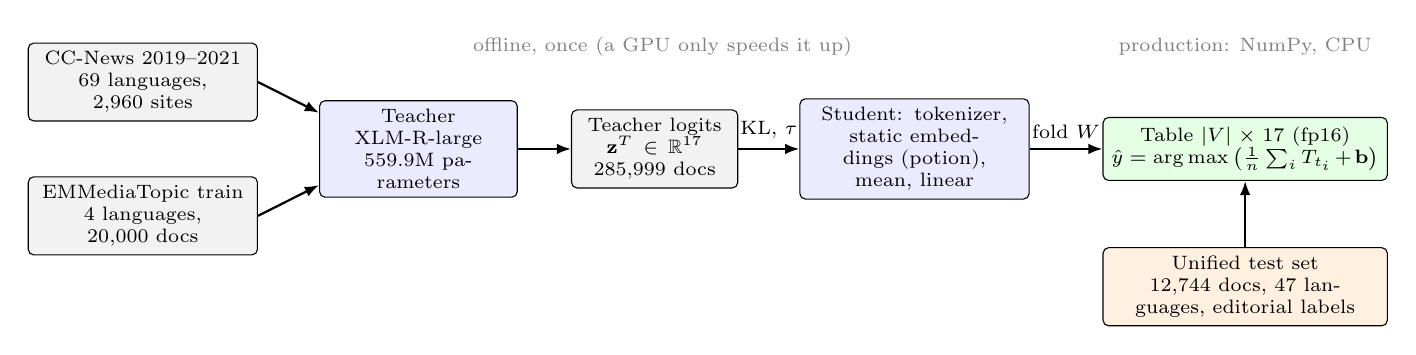
\begin{tikzpicture}[
  box/.style={draw, rounded corners=2pt, align=center, font=\scriptsize, inner sep=3pt, minimum height=8mm},
  data/.style={box, fill=gray!10},
  model/.style={box, fill=blue!8},
  prod/.style={box, fill=green!10},
  test/.style={box, fill=orange!12},
  arr/.style={-{Latex[length=1.8mm]}, thick},
  lab/.style={font=\scriptsize}]
  \node[data, text width=27mm] (cc)  at (1.4, 0.85)  {CC-News 2019--2021\\69 languages, 2,960 sites};
  \node[data, text width=27mm] (emm) at (1.4,-0.85)  {EMMediaTopic train\\4 languages, 20,000 docs};
  \node[model, text width=23mm] (t)  at (4.9, 0)     {Teacher\\XLM-R-large\\559.9M parameters};
  \node[data, text width=19mm] (soft) at (7.9, 0)    {Teacher logits\\$\mathbf{z}^{T}\in\mathbb{R}^{17}$\\285,999 docs};
  \node[model, text width=27mm] (s)  at (11.2, 0)    {Student: tokenizer,\\static embeddings (potion),\\mean, linear};
  \node[prod, text width=34mm] (tab) at (15.4, 0)    {Table $|V|\times 17$ (fp16)\\$\hat{y}=\arg\max\big(\frac{1}{n}\sum_i T_{t_i}+\mathbf{b}\big)$};
  \node[test, text width=34mm] (ts) at (15.4, -1.75)  {Unified test set\\12,744 docs, 47 languages, editorial labels};
  \draw[arr] (cc.east)  -- (t.160);
  \draw[arr] (emm.east) -- (t.200);
  \draw[arr] (t) -- (soft);
  \draw[arr] (soft) -- node[lab, above]{KL, $\tau$} (s);
  \draw[arr] (s) -- node[lab, above]{fold $W$} (tab);
  \draw[arr] (ts.north) -- (tab.south);
  \node[lab, text=gray] at (8.0, 1.3) {offline, once (a GPU only speeds it up)};
  \node[lab, text=gray] at (15.4, 1.3) {production: NumPy, CPU};
\end{tikzpicture}
\caption{StaticKD pipeline. The teacher labels an unlabeled news corpus once, offline. The student learns to imitate the teacher distribution, and its linear head is then folded into a token table, so inference only looks up and averages table rows. The final evaluation uses a test set whose labels do not come from the teacher.}
\label{fig:pipeline}
\end{figure*}

\subsection{Problem Formulation}
Given a news article $d$ in any language (title and body, truncated to the first 512 words as in~\cite{kuzman2025llm}), a model predicts one label $y\in\mathcal{Y}$ among the 17 top-level IPTC topics. The teacher $f_T$ outputs logits $\mathbf{z}^T(d)\in\mathbb{R}^{17}$. The goal is a student $f_S$ whose inference costs $O(n)$ additions for $n$ tokens and needs neither matrix multiplication nor a deep learning library. Its accuracy against independent labels should be as close as possible to that of $f_T$.

\subsection{Distillation Data and Development Set}
\label{sec:distdata}
The distillation data and the development set both draw on EMMediaTopic 1.0~\cite{emmediatopic2025,kuzman2025llm}, which Kuzman and Ljube\v{s}i\'c released together with the teacher model. EMMediaTopic was labeled with GPT-4o and consists of articles in four languages (Catalan, Greek, Croatian, and Slovenian). From these annotations, 21,000 articles were taken and divided into a training split of 20,000 articles and a development split of 1,000 articles. The training split is the data that Kuzman and Ljube\v{s}i\'c used to train the teacher, and this study uses it as part of the distillation data for the student. The development split was never used to train the teacher or the student. It was used to search for the hyperparameters of the teacher~\cite{kuzman2025llm}, and this study uses it as the development set for choosing the StaticKD recipe.

A large part of the distillation data comes from CC-News 2019--2021, a multilingual dataset~\cite{cloversearch_ccnews} built from the news archive of Common Crawl. In contrast, the test set was drawn from CC-News for a different range of years (CC-NEWS 2024--2026, Section~\ref{sec:testset}). CC-News 2019--2021 was processed with the following steps.
\begin{enumerate}
  \item Verify the language with the fastText language identification model~\cite{joulin2017bag} and keep only documents whose metadata language agrees with the identified language.
  \item Take the title and body if they have at least 75 words in total (200 characters for ja, zh, th, my), then truncate them to 512 words.
  \item Keep at most 150 documents per site.
  \item Form a held-out split by domain: all documents of some sites are set aside, with at most 20\% per language.
  \item Add 156,157 documents from training sites only (at most 5,000 per language and 400 per site).
\end{enumerate}
The distillation data contain 285,999 documents in 69 languages from 2,960 sites, with a median of 269 words. The number of documents per site is capped to avoid bias from similar content within one site. A few multilingual sites (for example bbc.com) were set aside in one language but also appear in the distillation data in another language, so their articles were removed from the held-out split. The resulting held-out set contains 12,554 documents in 63 languages from 217 sites that never occur in the distillation data. This set has no independent category labels, so it can only measure \emph{agreement} with the teacher. Agreement is the share of documents whose top predicted label is the same as the top label of the teacher.

\subsection{Unified Test Set Construction}
\label{sec:testset}
The first source is the CC-NEWS 2024--2026 dataset, sampled as one archive file (WARC) per month from January 2024 to August 2026 (32 files)~\cite{commoncrawl2026ccnews}. From each article page, the schema.org JSON-LD blocks~\cite{guha2016schema} supplied metadata fields such as \texttt{articleSection}, \texttt{BreadcrumbList}, \texttt{inLanguage}, \texttt{datePublished}, \texttt{isAccessibleForFree}, and \texttt{articleBody}. The text was taken from \texttt{articleBody} only when it had at least 30 words. Otherwise, the text was extracted from the HTML content with the Trafilatura library~\cite{barbaresi2021trafilatura}. Articles from sites that already appear in the distillation data or in an evaluation set were removed, which left 399,468 articles from new sites.

The second source is public datasets. MasakhaNEWS~\cite{adelani2023masakhanews} and MN-DS~\cite{petukhova2023mnds} are labeled by humans. L3Cube-IndicNews (LDC split)~\cite{mirashi2023indicnews}, Bangla news~\cite{hossain2025banglanews}, and IndoNews~\cite{indonews2021} carry publisher categories.

Section and category labels record where the newsroom placed an article when it was published. Such labels are called \emph{editorial labels} in this paper. Editorial labels do not follow the IPTC standard, so the section names have to be translated onto the official IPTC Media Topic tree (1,085 active nodes). The process starts by normalizing the section names (case, diacritics) and continues with a conservative mapping by an LLM (Claude Opus 5.5). A name is mapped only if the content under that section fits a single top-level topic. As a result, 814 section names were mapped to 79 IPTC nodes. An automatic check verifies that every target node exists in the IPTC tree, is not retired, and lies under the intended top-level topic. Articles whose sections map to different labels are rejected. The first author then reviewed each rule of the mapping table drafted by the LLM to ensure its accuracy. This review covered 916 rules, namely 814 valid mapped names and 102 ambiguous, language-specific, and rejecting rules.

Quality and leakage filters are applied in order.
\begin{enumerate}
  \item Publication date on or after 1 January 2024 (CC-NEWS only).
  \item Not behind a paywall.
  \item Declared language agrees with fastText language identification when fastText supports the language.
  \item At least 75 words.
  \item Deduplication of uniform resource locators (URLs), identical texts, and near-duplicates (MinHash~\cite{broder1997resemblance}, Jaccard $\ge 0.7$~\cite{lee2022dedup}) across all sources.
  \item Contamination: an article is dropped when $\ge 30\%$ of its word 8-grams occur in any of about 300 thousand training or evaluation documents. This filter removed 50 articles, mostly from MasakhaNEWS, which also draws on BBC.
\end{enumerate}

Sampling takes at most 50 articles for each pair of language and label. Human-labeled sources have priority, followed by publisher categories and then JSON-LD sections. The number of articles per site is not capped. Languages with fewer than 30 articles are dropped. Articles from the same site tend to be similar, so whole sites are resampled when confidence intervals are computed (Section~\ref{sec:protocol}). Section~\ref{sec:res-acc} also repeats the comparison with at most five articles per site.

The final test set contains 12,744 articles in 47 languages from 1,227 sites or sources. All 17 labels occur in it, and the median article length is 313 words. Human annotators labeled 4,094 of these articles (32.1\%). Publisher categories cover 2,600 (20.4\%) and JSON-LD sections 6,050 (47.5\%). The label type of an article (human annotation, publisher category, or JSON-LD section) is called its \emph{label origin}. No distillation data exist for 13 languages (e.g., ha, yo, ig, bn, and pa). Another 9 languages have fewer than 500 distillation documents, and 25 have at least 500. Site diversity is measured by the effective number of sites, $1/\sum_s q_s^{2}$, where $q_s$ is the share of the articles of a language that come from site $s$. A source dataset without URLs counts as one site. By this measure, 13 languages have at least 10 effective sites, while 27 languages practically come from only one publisher. Table~\ref{tab:testset} summarizes the composition of the article sources and Fig.~\ref{fig:testset} shows the number of articles of each language per label.

\begin{table}[!t]
\caption{Composition of the Unified Test Set by Source}
\label{tab:testset}
\centering
\footnotesize
\setlength{\tabcolsep}{3pt}
\resizebox{\columnwidth}{!}{%
\begin{tabular}{@{}llrrr@{}}
\toprule
Source & Label origin & Articles & Languages & Sites/sources \\
\midrule
CC-NEWS 2024--2026 & JSON-LD section & 6,050 & 29 & 1,092 \\
MasakhaNEWS~\cite{adelani2023masakhanews} & human annotation & 3,339 & 16 & 6 \\
L3Cube-IndicNews~\cite{mirashi2023indicnews} & publisher category & 2,361 & 10 & 1 \\
MN-DS~\cite{petukhova2023mnds} & human annotation & 755 & 1 & 127 \\
Bangla news~\cite{hossain2025banglanews} & publisher category & 139 & 1 & 1 \\
IndoNews & publisher category & 100 & 1 & 1 \\
\midrule
Total & & 12,744 & 47 & 1,227 \\
\bottomrule
\end{tabular}}
\end{table}

\begin{figure}[!t]
\centering
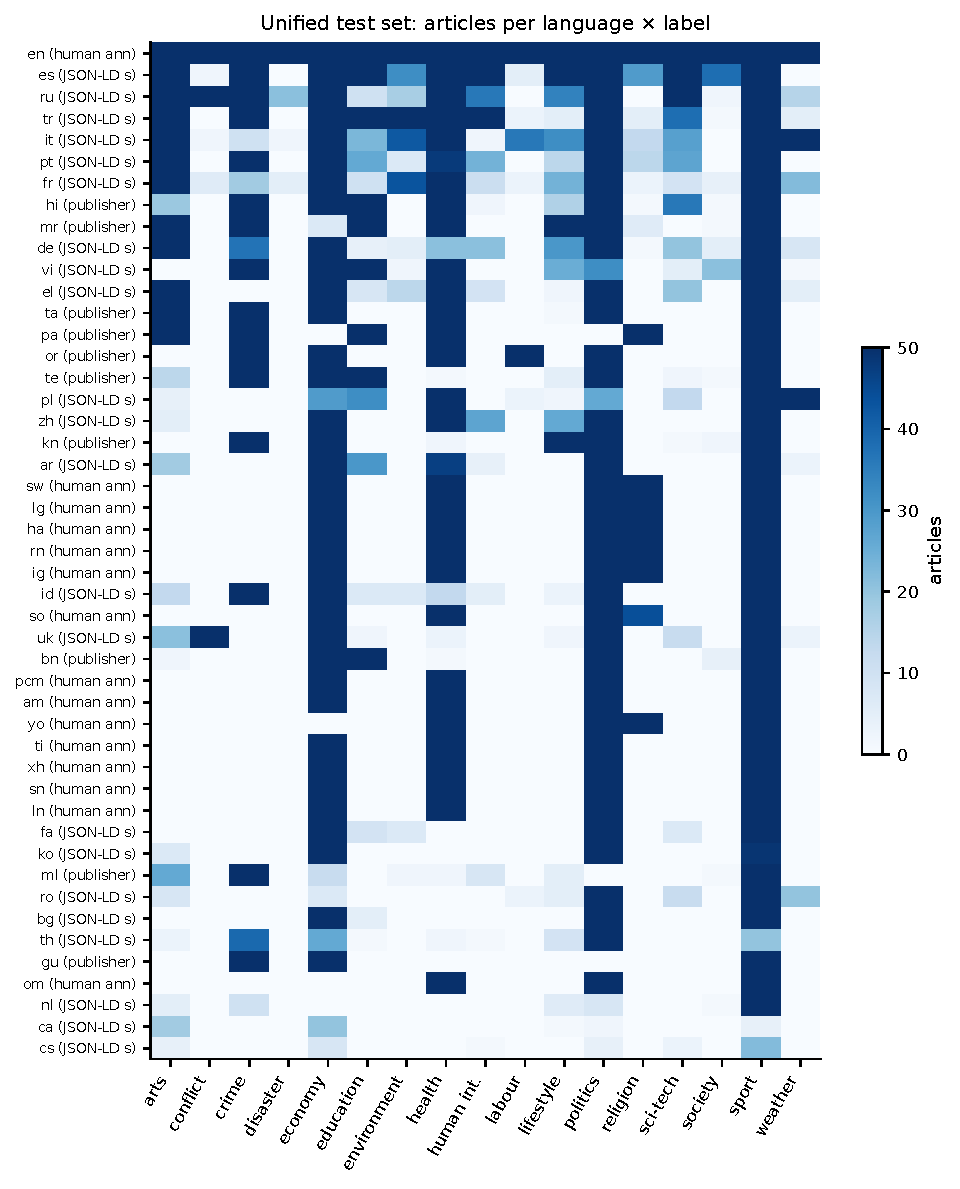
\includegraphics[width=\columnwidth]{figures/fig_testset_heatmap.pdf}
\caption{Articles in the unified test set per language and label (at most 50 per language--label pair). The label origin in brackets is the dominant one for that language.}
\label{fig:testset}
\end{figure}

\subsection{Teacher and Distillation Labels}
\label{sec:teacher}
The teacher is the IPTC classifier of~\cite{kuzman2025llm}, published as \url{classla/multilingual-IPTC-news-topic-classifier}. It is an XLM-RoBERTa-large model with 24 layers, 559.9 million parameters, and an input limit of 512 XLM-R tokens. For 60.7\% of the test articles, the 512-word input exceeds this limit. On those articles the teacher reads about 287 of 438 words (medians). For every distillation document, the teacher produces a logit vector $\mathbf{z}^{T}(d)\in\mathbb{R}^{17}$, which is stored in full. Labeling was run once in fp16 on an NVIDIA RTX~4050 Laptop GPU (6~GB), with batches sorted by text length. Measured on a fixed sample of 5,000 documents, the teacher labels 50.1 documents per second, so labeling all distillation data takes about 1.58 GPU hours. The teacher label distribution on CC-News 2019--2021 is plausible (\emph{politics} 16.5\%, \emph{economy} 12.7\%, \emph{sport} 11.6\%, \emph{weather} 1.3\%), and the mean confidence per language ranges from 0.90 to 1.00.

\subsection{The StaticKD Student}
\label{sec:student}
The student in this study is built on the multilingual static embedding model potion-multilingual-128M of Model2Vec~\cite{tulkens2024model2vec}, hereafter called potion. A document $d$ is tokenized into $t_1,\dots,t_n$ with the Unigram tokenizer of potion, which contains 500,353 tokens, so that every token has a pre-trained embedding. Special tokens are not used, and unknown tokens are dropped. The document length is capped at 1,024 tokens. Because averaging does not depend on position, this cap only serves to bound the cost. Only 5.4\% of the test articles exceed it. Each token has an embedding $\mathbf{e}_t\in\mathbb{R}^{256}$, and
\begin{equation}
\mathbf{h}(d)=\frac{1}{n}\sum_{i=1}^{n}\mathbf{e}_{t_i},\qquad
\mathbf{z}^{S}(d)=W\,\mathrm{drop}(\mathbf{h}(d))+\mathbf{b},
\label{eq:student}
\end{equation}
with $W\in\mathbb{R}^{17\times 256}$ and dropout 0.1 during training. The embedding matrix $E$ is initialized from potion. The potion model itself obtains its embeddings for 101 languages through distillation from BGE-M3~\cite{chen2024bgem3}. With this initialization, the tokens of these 101 languages already lie in one shared space before training starts. The comparison with a random initialization is given in Section~\ref{sec:res-abl}.

The student learns from the stored teacher logits with the loss
\begin{equation}
\mathcal{L}_{\mathrm{KD}}=\tau^{2}\,\mathrm{KL}\!\left(p^{T}\,\middle\|\,p^{S}\right),\qquad \tau=1 ,
\label{eq:kd}
\end{equation}
where $p^{T}=\mathrm{softmax}(\mathbf{z}^{T}/\tau)$ and $p^{S}=\mathrm{softmax}(\mathbf{z}^{S}/\tau)$ are the teacher and student distributions, respectively. The value $\tau=1$ was chosen during development, and the results for $\tau\in\{0.5,2,4\}$ are reported in Section~\ref{sec:res-abl}. The parameters $E$, $W$, and $\mathbf{b}$ are trained together. The embedding matrix $E$ uses SparseAdam ($\eta=10^{-3}$), which updates only the rows of tokens that occur in the current batch. Tokens that never occur in the training documents therefore keep their potion embeddings, and Section~\ref{sec:discussion} returns to this property. AdamW ($\eta=3\cdot 10^{-3}$, weight decay $10^{-4}$) is used for $W$ and $\mathbf{b}$. Training runs for 6 epochs with a batch size of 64. A cheap augmentation in the form of token dropout is also applied. At every step, each token of a training document is dropped with probability 0.2 so that the model does not rely on a few keywords. Internal validation uses 3\% of the distillation data (8,579 documents), and the epoch with the highest agreement with the teacher is kept.

The classification head is linear, so \eqref{eq:student} can be rewritten as
\begin{equation}
W\Big(\frac{1}{n}\sum_{i}\mathbf{e}_{t_i}\Big)+\mathbf{b}=\frac{1}{n}\sum_{i}T_{t_i}+\mathbf{b},
\label{eq:fold}
\end{equation}
with the table $T=EW^{\top}\in\mathbb{R}^{|V|\times 17}$. The folding step computes $T$ once after training. Row $T_t$ holds the 17 topic scores that token $t$ contributes to every article that contains it. For production, the model consists only of $T$ (fp16), $\mathbf{b}$, and the tokenizer. Algorithm~\ref{alg:infer} lists the whole inference procedure. The same argument also holds for an ensemble. Equation~\eqref{eq:fold} is linear in $T$, so averaging the logits of $K$ students trained with different seeds gives the same result as one student with table $\bar{T}=\frac{1}{K}\sum_k T^{(k)}$ and bias $\bar{\mathbf{b}}$. During development, the student was trained with three seeds (0, 1, and 2), and the final StaticKD model averages the tables of these three seeds ($K=3$). It has 8.5 million parameters and a size of 34~MB.

\begin{algorithm}[!t]
\caption{StaticKD Inference for One Article}
\label{alg:infer}
\begin{algorithmic}[1]
\Require article text $d$; tokenizer; table $\bar{T}\in\mathbb{R}^{|V|\times 17}$; bias $\bar{\mathbf{b}}\in\mathbb{R}^{17}$
\State $(t_1,\dots,t_n)\gets$ first 1,024 tokens of tokenize$(d)$, without unknown tokens
\State $\mathbf{z}\gets\frac{1}{n}\sum_{i=1}^{n}\bar{T}_{t_i}+\bar{\mathbf{b}}$ \Comment{look up and average table rows}
\State \Return $\arg\max_{y}\,z_y$ \Comment{one of the 17 IPTC topics}
\end{algorithmic}
\end{algorithm}

The table itself takes 16~MB, but the internal structure of the Unigram tokenizer needs much more random-access memory (RAM). A compact variant shrinks this structure by removing token pieces that occur fewer than 10 times in the distillation data. Single characters are kept. The vocabulary of this variant has 335,441 tokens, and the model size is 23~MB. The hyperparameters of all models are listed in Table~\ref{tab:hparams}.

\begin{table}[!t]
\caption{Hyperparameters of All Models}
\label{tab:hparams}
\centering
\footnotesize
\setlength{\tabcolsep}{3pt}
\resizebox{\columnwidth}{!}{%
\begin{tabular}{@{}ll@{}}
\toprule
Component & Value \\
\midrule
\multicolumn{2}{@{}l}{\textit{StaticKD}} \\
\quad initial embedding & potion-multilingual-128M (500,353 $\times$ 256) \\
\quad max. tokens / vector dropout & 1,024 / 0.1 \\
\quad loss, $\tau$ & KL, $\tau=1$ \\
\quad token dropout & 0.2 \\
\quad optimizer embedding / head & SparseAdam $10^{-3}$ / AdamW $3\cdot 10^{-3}$, wd $10^{-4}$ \\
\quad batch, epoch, validation & 64, 6, 3\% of data (selects the epoch) \\
\quad ensemble & mean of 3 seed tables \\
\multicolumn{2}{@{}l}{\textit{fastText}} \\
\quad word tokens (fixed) & dim 100, lr 0.5, 15 epoch \\
\quad subword tokens (fixed) & dim 100, lr 0.5, 15 epoch \\
\quad GPT-4o labels & dim 100, lr 0.5, 25 epoch \\
\quad word n-grams, loss & 2, softmax, 2M buckets \\
\quad tokens & words (+ character 2--5-grams) or XLM-R subwords \\
\quad quantization & \texttt{quantize}, cutoff 300k, retrain \\
\multicolumn{2}{@{}l}{\textit{TF-IDF + SVM}} \\
\quad features & XLM-R subword uni+bigrams, min.\ df 3, max.\ 1,000,000, sublinear tf \\
\quad classifier (fixed) & LinearSVC, $C=0.50$ \\
\multicolumn{2}{@{}l}{\textit{MiniLM-L6 / DistilmBERT + KD}} \\
\quad optimizer & AdamW $5\cdot 10^{-5}$, wd 0.01, warmup 6\%, linear, fp16 \\
\quad batch, epoch, max. tokens & 32, 2, 256 \\
\quad $\tau$ & $\{1, 2\}$, chosen on dev \\
\bottomrule
\end{tabular}}
\end{table}

\subsection{Baselines}
\label{sec:baselines}
All baselines marked + KD use the same distillation data (285,999 documents) and targets from the same teacher. fastText + KD~\cite{joulin2017bag} is trained on the top teacher label, with word tokens (plus character n-grams) or with XLM-R subwords. Its quantized variant (\texttt{.ftz}) is included as well. A fastText model is also trained only on the GPT-4o labels of the EMMediaTopic training split and serves as a reference with labeled data equivalent to that available to~\cite{kuzman2025llm}. The non-neural baseline TF-IDF + SVM + KD comes from Kuzman and Ljube\v{s}i\'c. This model uses TF-IDF features with a support vector classifier and is trained on the top teacher label over XLM-R subwords. For the non-transformer baselines, the hyperparameters were set once without a search. Their values are listed in Table~\ref{tab:hparams}. MiniLM-L6 + KD uses mMiniLMv2-L6-H384, which is distilled from XLM-R-large~\cite{wang2021minilmv2}. The temperature $\tau\in\{1,2\}$ for this model was chosen on the development set. The same recipe is applied to DistilmBERT + KD with \texttt{distilbert-base-multilingual-cased}~\cite{sanh2019distilbert}. Both transformers read at most 256 tokens. As a result, 91.1\% of the test articles are truncated to about 142 words for MiniLM-L6, while for DistilmBERT 93.2\% of the articles are truncated to about 116 words. Both are exported to ONNX fp32 for the CPU benchmark. The ONNX int8 teacher is an export of the teacher with dynamic int8 quantization and is the fastest teacher configuration on CPU.

Among prior studies, Sparse Distillation~\cite{ye2022sparse} is the closest to StaticKD. This method and the classifier trainer of Model2Vec were not run as separate baselines. The decision is discussed further in Section~\ref{sec:limitations}. Even so, parts of both are still covered. fastText + KD is a bag-of-n-grams model with averaging and a linear head, and it is trained on the same teacher labels. In the random-initialization ablation (Section~\ref{sec:design}), the embedding table is trained from scratch, as in Sparse Distillation. The frozen-embedding ablation trains only a linear head on top of potion, so this ablation acts as an off-the-shelf Model2Vec baseline with a distilled head.

\subsection{Evaluation Protocol and Statistical Tests}
\label{sec:protocol}
The label distribution is imbalanced, so the main metric is macro-F1 over the labels present in the reference. It is computed in the same way as in the evaluation code of~\cite{kuzman2025llm}. The evaluation also reports accuracy, agreement with the teacher on the held-out set, and macro-F1 per language. The per-language macro-F1 is averaged over languages so that large languages do not dominate.

The 95\% confidence intervals come from a percentile bootstrap of 1,000 resamples. On the test set, the resampling unit is the site, or the source dataset when an article has no URL. Such a site-cluster bootstrap~\cite{field2007bootstrapping} draws whole sites. Related articles from one site are drawn together and are not treated as independent data, so the intervals do not become too narrow. On the development set, the unit is the document. Two models tested on the same documents are compared with a paired (cluster) bootstrap of 2,000 resamples for $\Delta$macro-F1~\cite{koehn2004significance} and an exact McNemar test for accuracy~\cite{mcnemar1947}. Holm correction~\cite{holm1979} is applied within each set. Each ablation variant is run with five seeds, while the final recipe is run with ten. Differences between variants are tested with Welch tests at the seed level and then Holm-corrected. Whether a difference is consistent across languages is checked with a Wilcoxon signed-rank test on per-language macro-F1 and accuracy~\cite{dror2018hitchhiker}. Subgroup analyses split the results by language, script, and region. Further splits use the label and its origin. The remaining subgroups are defined by site diversity, the amount of distillation data of the language, and teacher pre-training coverage. Pre-training coverage refers to whether the language is among the 100 languages used to pre-train XLM-R~\cite{conneau2020xlmr}. The relation between per-language properties and performance is measured with Spearman correlations, while a Kruskal--Wallis test is used to compare scripts. This analysis uses two per-language quantities. The \emph{accuracy gap} is the StaticKD accuracy minus the teacher accuracy, so a negative gap means that StaticKD is less accurate. The \emph{token coverage} of a language is computed over all token occurrences in its test articles. Its value is the share of occurrences whose token occurs at least 10 times in the distillation data. The embeddings of rarer tokens are rarely updated during training (Section~\ref{sec:student}). Calibration is measured with the expected calibration error (ECE, 15 bins)~\cite{guo2017calibration}, because the cascade mode in Section~\ref{sec:effprotocol} routes articles by the confidence of StaticKD.

\subsection{Efficiency Protocol}
\label{sec:effprotocol}
The benchmark runs only on CPU, and the GPU is hidden. Each model runs in a fresh process, and the thread count is pinned in every library (OMP, MKL, OpenBLAS, ONNX Runtime, \texttt{tokenizers}). Latency (p50 and p95) is measured with one article per call, as in a streaming setting. Throughput is measured with batches of 64, or 8 for transformers. Model RAM is the increase in resident set size after the model is loaded. All models use the same text sample, drawn at random from the unified test set. The teacher and the transformers use 30 documents for latency and 48 documents for throughput, while the light models use 500 and 3,000 documents. All models are measured in one session on an idle machine. The teacher stops at 512 tokens, whereas StaticKD reads up to 1,024 tokens per article, so the speed comparison does not favor StaticKD. In cascade mode, StaticKD decides the articles on which its top probability is at least a threshold $\theta$. The remaining articles are passed to the ONNX int8 teacher. Let $s$ be the share of articles decided by StaticKD, and let $r_S$ and $r_T$ be the single-core throughputs of StaticKD and the teacher. The effective throughput of the cascade is then $1/(1/r_S+(1-s)/r_T)$.

The machine is a laptop with an Intel Core Ultra~7 155H, 31~GB of RAM, and Windows~11. Its CPU is hybrid and has 6 performance cores (P-cores), 8 slower efficiency cores (E-cores), and 2 low-power E-cores. If threads are not pinned, the operating system moves them to the slow cores. Each process is therefore pinned to physical P-cores: logical CPU 0 for one core and logical CPUs 0, 10, 12, and 14 for four cores. This setup approximates a small server with uniform cores.

\subsection{Experimental Design and Implementation Details}
\label{sec:design}
The final recipe and its ablations comprise 60 runs, all of which are listed in Table~\ref{tab:ablation}. Each ablation variant changes one factor of the final recipe. One variant replaces the soft labels with hard labels. Two variants reduce the training data, either to EMMediaTopic only (4 languages, 10 epochs) or to 130 thousand documents without the extra CC-News 2019--2021 data. Other variants initialize the embeddings randomly with the same standard deviation as potion or keep them frozen. The remaining variants train without token dropout, use a 512-unit multilayer perceptron (MLP) head, or set $\tau\in\{0.5,\,2,\,4\}$. During development, twelve further runs tested four additions to the recipe, each with three seeds. The four additions are bigram features, idf-weighted pooling, documents weighted by teacher confidence, and an extra loss on the GPT-4o labels. None of the additions differs significantly from the final recipe on the development set, and none of them changes the test macro-F1 by more than 0.004. These additions are therefore left out of both the recipe and Table~\ref{tab:ablation}. On average, one StaticKD run takes 5.2 minutes on the same GPU. The implementation uses Python~3.12, NumPy~2.5, PyTorch~2.6, transformers~5.17, \texttt{tokenizers}~0.23, ONNX Runtime~1.30, scikit-learn~1.9, and fastText~0.9.2. The seed, library versions, and training history of every run are stored with the model.

\section{Results}
\label{sec:results}
\subsection{Accuracy of All Models (RQ1)}
\label{sec:res-acc}
\begin{table*}[!t]
\caption{Main Results. Macro-F1 [95\% CI] and Accuracy on the Development Set (EMMediaTopic Dev, GPT-4o Labels), Agreement with the Teacher on CC-News Held-Out, and Results on the Unified Test Set (47 Languages, Independent Labels). Test CIs from the Site-Cluster Bootstrap}
\label{tab:main}
\centering
\footnotesize
\setlength{\tabcolsep}{3.5pt}
\begin{tabular}{@{}lccccccc@{}}
\toprule
 & \multicolumn{2}{c}{dev (4 languages)} & held-out & \multicolumn{4}{c}{unified test (47 languages)} \\
\cmidrule(lr){2-3}\cmidrule(lr){4-4}\cmidrule(lr){5-8}
Model & Macro-F1 [95\% CI] & Accuracy & Agreement & Macro-F1 [95\% CI] & Accuracy & Macro-F1/language & \% teacher \\
\midrule
Teacher XLM-R-large & 0.822 [0.779--0.851] & 0.859 & -- & 0.598 [0.546--0.643] & 0.700 & 0.705 & 100.0\% \\
Teacher XLM-R-large, ONNX int8 & 0.823 [0.781--0.852] & 0.858 & -- & 0.600 [0.547--0.646] & 0.699 & 0.702 & 100.3\% \\
\midrule
DistilmBERT + KD & 0.753 [0.710--0.785] & 0.801 & 0.799 & 0.534 [0.481--0.618] & 0.623 & 0.602 & 89.4\% \\
MiniLM-L6 + KD & 0.785 [0.737--0.815] & 0.820 & 0.825 & 0.566 [0.511--0.624] & 0.667 & 0.661 & 94.6\% \\
\midrule
\textbf{StaticKD (proposed)} & \textbf{0.761 [0.717--0.792]} & 0.800 & 0.811 & \textbf{0.545 [0.490--0.605]} & 0.641 & 0.622 & 91.1\% \\
StaticKD-compact & 0.754 [0.710--0.786] & 0.797 & 0.802 & 0.484 [0.421--0.597] & 0.544 & 0.507 & 81.0\% \\
\midrule
fastText + KD, subword, quantized & 0.708 [0.664--0.739] & 0.759 & 0.740 & 0.435 [0.370--0.556] & 0.512 & 0.464 & 72.7\% \\
fastText + KD, subword & 0.727 [0.691--0.756] & 0.769 & 0.751 & 0.445 [0.384--0.563] & 0.522 & 0.473 & 74.4\% \\
fastText + KD, word & 0.743 [0.707--0.773] & 0.789 & 0.753 & 0.438 [0.373--0.560] & 0.511 & 0.472 & 73.3\% \\
TF-IDF + SVM + KD & 0.755 [0.719--0.786] & 0.798 & 0.776 & 0.486 [0.431--0.585] & 0.567 & 0.522 & 81.3\% \\
\midrule
fastText, GPT-4o labels, subword & 0.665 [0.613--0.700] & 0.729 & 0.260 & 0.086 [0.069--0.119] & 0.150 & 0.118 & 14.4\% \\
fastText, GPT-4o labels, word & 0.651 [0.601--0.693] & 0.738 & 0.307 & 0.106 [0.085--0.150] & 0.181 & 0.142 & 17.7\% \\
\bottomrule
\end{tabular}
\end{table*}
On the unified test set, StaticKD keeps 91.1\% of the teacher macro-F1. Its score is 0.545 [0.490--0.605], against 0.598 [0.546--0.643] for the teacher (Table~\ref{tab:main}). Both scores are far lower than the development scores (0.761 and 0.822) because most of the test set lies outside the languages, sources, and period of the data used to train the teacher. On the development set, StaticKD keeps 92.6\% of the teacher score. For the 63 held-out languages, the predictions of StaticKD match those of the teacher on 81.1\% of the documents. Without ensembling, a single student reaches 0.542 $\pm$ 0.004 on the test set (10 seeds).

MiniLM-L6 starts from a distillation of XLM-R-large, and its score (0.566) lies between StaticKD and the teacher. DistilmBERT (0.534) is on par with StaticKD, although its cost is much higher. Two baselines have a cost similar to that of StaticKD: fastText + KD and TF-IDF + SVM + KD. Both fall below StaticKD. The last two rows show what happens when there are no teacher labels for other languages. fastText trained only on the GPT-4o labels of four languages reaches 0.665 on the development set but only 0.086 on the test set.

\begin{table*}[!t]
\caption{Paired Tests of StaticKD Against Other Models on the Unified Test Set. $\Delta$ = StaticKD $-$ Comparison Model. $p$ Is Holm-Corrected Over the Comparisons. $b/c$ = Documents Correct Only for StaticKD / Only for the Comparison Model}
\label{tab:sig}
\centering
\footnotesize
\begin{tabular}{@{}lccccc@{}}
\toprule
StaticKD vs & $\Delta$macro-F1 [95\% CI] & $p$ bootstrap & $\Delta$accuracy & McNemar $b/c$ & $p$ McNemar \\
\midrule
Teacher XLM-R-large & $-$0.053 [$-$0.065, $-$0.033] & $<$0.001 & $-$0.059 & 654/1400 & $<$0.001 \\
Teacher XLM-R-large, ONNX int8 & $-$0.055 [$-$0.067, $-$0.035] & $<$0.001 & $-$0.058 & 644/1386 & $<$0.001 \\
DistilmBERT + KD & +0.010 [$-$0.026, +0.041] & 0.800 & +0.018 & 1372/1143 & $<$0.001 \\
MiniLM-L6 + KD & $-$0.021 [$-$0.038, $-$0.008] & 0.004 & $-$0.026 & 866/1197 & $<$0.001 \\
StaticKD-compact & +0.060 [+0.003, +0.100] & 0.030 & +0.097 & 1345/110 & $<$0.001 \\
fastText + KD, subword, quantized & +0.110 [+0.042, +0.151] & $<$0.001 & +0.129 & 2157/519 & $<$0.001 \\
fastText + KD, subword & +0.100 [+0.037, +0.138] & $<$0.001 & +0.119 & 2021/505 & $<$0.001 \\
fastText + KD, word & +0.106 [+0.041, +0.149] & $<$0.001 & +0.130 & 2176/513 & $<$0.001 \\
TF-IDF + SVM + KD & +0.059 [+0.009, +0.093] & 0.030 & +0.074 & 1667/719 & $<$0.001 \\
fastText, GPT-4o labels, subword & +0.458 [+0.415, +0.496] & $<$0.001 & +0.491 & 6597/344 & $<$0.001 \\
fastText, GPT-4o labels, word & +0.439 [+0.393, +0.475] & $<$0.001 & +0.460 & 6252/391 & $<$0.001 \\
\bottomrule
\end{tabular}
\end{table*}
The paired tests in Table~\ref{tab:sig} confirm this ranking. The $\Delta$macro-F1 of StaticKD against the teacher is $-$0.053 [$-$0.065, $-$0.033]. Against MiniLM-L6, the difference is $-$0.021 [$-$0.038, $-$0.008] with $p=0.004$. The difference from DistilmBERT is not significant (+0.010, $p=0.800$). StaticKD is indeed correct on more test articles than DistilmBERT (McNemar $p<0.001$). However, the McNemar test treats every article as independent and does not account for the dependence between articles from the same site. StaticKD is ahead of the quantized fastText + KD by +0.110 [+0.042, +0.151]. Its advantage over TF-IDF + SVM is +0.059 [+0.009, +0.093] ($p=0.030$).

The macro-F1 of StaticKD is higher than that of fastText + KD in 43 of 47 languages (Wilcoxon $p<0.001$). The advantage over this baseline thus holds in almost every language. The advantage over TF-IDF + SVM is narrower. In macro-F1, StaticKD is ahead in 31 of 47 languages (Wilcoxon $p=0.003$). Per-language accuracy gives a different picture, with StaticKD higher in 24 languages and lower in 22 (Wilcoxon $p=0.127$), so the accuracy of the two models is close. Neither metric differs consistently across languages when StaticKD is compared with DistilmBERT (Wilcoxon $p=0.604$ for macro-F1 and 0.322 for accuracy). StaticKD beats the teacher in only 7 of 47 languages.

Table~\ref{tab:groups} and Fig.~\ref{fig:groups} show that the share of the teacher score that StaticKD keeps varies far more with the amount of distillation data in the language of the article than with the type of label. By label origin, the share ranges from 89.5\% for publisher categories to 95.8\% for JSON-LD sections. By the amount of distillation data in the language, the share falls from 97.5\% in languages with at least 500 documents to 72.3\% in languages without distillation data. A test set limited to at most five articles per site and language--label pair gives the same model ranking. On this subset of 8,139 articles, StaticKD obtains 0.587 and the teacher 0.627.

\begin{table*}[!t]
\caption{Test Macro-F1 by Subgroup. Last Column: StaticKD Macro-F1 as a Percentage of the Teacher Macro-F1 in the Same Subgroup}
\label{tab:groups}
\centering
\footnotesize
\setlength{\tabcolsep}{3.5pt}
\begin{tabular}{@{}lrcccccccc@{}}
\toprule
Subgroup & $n$ & Teacher & DistilmBERT & MiniLM & \textbf{StaticKD} & fastText (q) & TF-IDF+SVM & fastText GPT & \% teacher \\
\midrule
\multicolumn{10}{@{}l}{\textit{Label origin}} \\
\quad human annotation & 4,094 & 0.463 & 0.436 & 0.436 & 0.414 & 0.336 & 0.393 & 0.027 & 90\% \\
\quad publisher category & 2,600 & 0.702 & 0.498 & 0.674 & 0.629 & 0.319 & 0.330 & 0.063 & 90\% \\
\quad JSON-LD section & 6,050 & 0.651 & 0.629 & 0.634 & 0.624 & 0.579 & 0.609 & 0.136 & 96\% \\
\multicolumn{10}{@{}l}{\textit{Distillation data of the language}} \\
\quad sufficient ($\ge$500) & 7,644 & 0.633 & 0.617 & 0.616 & 0.618 & 0.572 & 0.593 & 0.116 & 98\% \\
\quad few ($<$500) & 2,243 & 0.537 & 0.344 & 0.496 & 0.478 & 0.202 & 0.227 & 0.037 & 89\% \\
\quad none (0) & 2,857 & 0.557 & 0.452 & 0.502 & 0.402 & 0.174 & 0.230 & 0.048 & 72\% \\
\multicolumn{10}{@{}l}{\textit{Region}} \\
\quad Africa & 3,044 & 0.697 & 0.532 & 0.576 & 0.542 & 0.312 & 0.408 & 0.085 & 78\% \\
\quad South Asia & 2,681 & 0.575 & 0.410 & 0.544 & 0.509 & 0.246 & 0.276 & 0.046 & 88\% \\
\quad East/Southeast Asia \& Middle East & 1,574 & 0.636 & 0.620 & 0.621 & 0.622 & 0.560 & 0.629 & 0.085 & 98\% \\
\quad Europe & 5,445 & 0.653 & 0.637 & 0.638 & 0.638 & 0.595 & 0.610 & 0.136 & 98\% \\
\multicolumn{10}{@{}l}{\textit{Teacher pre-training coverage}} \\
\quad outside XLM-R pre-training & 1,750 & 0.719 & 0.586 & 0.620 & 0.501 & 0.317 & 0.457 & 0.086 & 70\% \\
\quad in XLM-R pre-training & 10,994 & 0.609 & 0.549 & 0.585 & 0.576 & 0.468 & 0.503 & 0.096 & 95\% \\
\multicolumn{10}{@{}l}{\textit{Site diversity}} \\
\quad diverse ($\ge$10) & 5,225 & 0.657 & 0.642 & 0.643 & 0.642 & 0.598 & 0.616 & 0.134 & 98\% \\
\quad single publisher ($<$3) & 6,204 & 0.517 & 0.387 & 0.475 & 0.433 & 0.221 & 0.287 & 0.045 & 84\% \\
\quad medium (3--10) & 1,315 & 0.559 & 0.556 & 0.539 & 0.543 & 0.503 & 0.533 & 0.089 & 97\% \\
\bottomrule
\end{tabular}
\end{table*}

Table~\ref{tab:sources} splits the test set by source. MN-DS is the only source that is annotated directly with IPTC topics. On MN-DS, StaticKD keeps 97.4\% of the teacher score (0.535 against 0.549). The macro-F1 of the teacher itself is lower on this source than on any other source. StaticKD keeps the smallest share on MasakhaNEWS (80.0\%). The human labels of MasakhaNEWS follow a non-IPTC scheme, and 10 of its 16 languages are absent from the distillation data. Bangla is also absent from the distillation data, and Bangla news shows most clearly what the pre-trained embeddings contribute. There, fastText + KD and TF-IDF + SVM collapse to 0.150 and 0.010, while StaticKD reaches 0.748.

\begin{table*}[!t]
\caption{Test Macro-F1 by Source of the Unified Test Set. MN-DS Is the Only Source Annotated Directly With IPTC Topics. MasakhaNEWS Is Human-Annotated Under Its Own Scheme. Last Column: StaticKD as a Percentage of the Teacher}
\label{tab:sources}
\centering
\footnotesize
\setlength{\tabcolsep}{3.5pt}
\resizebox{\textwidth}{!}{\begin{tabular}{@{}llrrccccccc@{}}
\toprule
Source & Label origin & $n$ & Lang. & Teacher & DistilmBERT & MiniLM & \textbf{StaticKD} & fastText (q) & TF-IDF+SVM & \% teacher \\
\midrule
CC-NEWS 2024--2026 & JSON-LD section & 6,050 & 29 & 0.651 & 0.629 & 0.634 & 0.624 & 0.579 & 0.609 & 96\% \\
MasakhaNEWS~\cite{adelani2023masakhanews} & human annotation & 3,339 & 16 & 0.695 & 0.545 & 0.582 & 0.556 & 0.341 & 0.434 & 80\% \\
L3Cube-IndicNews~\cite{mirashi2023indicnews} & publisher category & 2,361 & 10 & 0.709 & 0.501 & 0.680 & 0.639 & 0.328 & 0.342 & 90\% \\
MN-DS~\cite{petukhova2023mnds} & human annotation & 755 & 1 & 0.549 & 0.546 & 0.535 & 0.535 & 0.493 & 0.461 & 97\% \\
Bangla news~\cite{hossain2025banglanews} & publisher category & 139 & 1 & 0.835 & 0.730 & 0.817 & 0.748 & 0.150 & 0.010 & 90\% \\
IndoNews & publisher category & 100 & 1 & 0.885 & 0.846 & 0.856 & 0.862 & 0.852 & 0.873 & 97\% \\
\bottomrule
\end{tabular}}
\end{table*}

\begin{figure*}[!t]
\centering
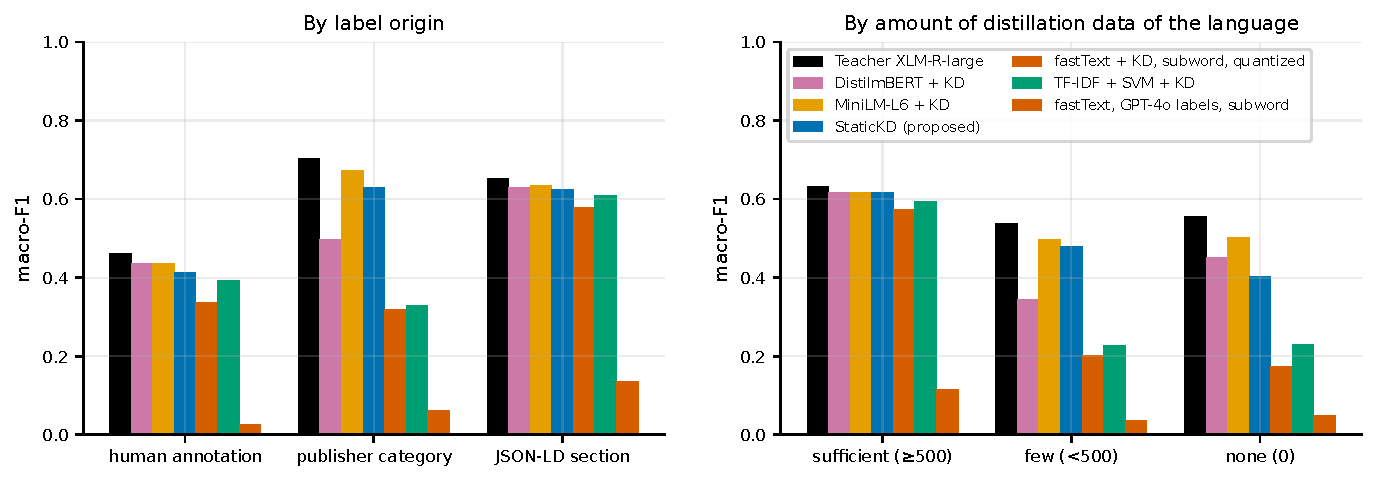
\includegraphics[width=0.78\textwidth]{figures/fig_groups.pdf}
\caption{Test macro-F1 by label origin (left) and by the amount of distillation data in the language of the article (right).}
\label{fig:groups}
\end{figure*}

\subsection{Validity of the Editorial Labels}
\label{sec:res-validity}
Two thirds of the test labels are section and category labels, which record newsroom decisions rather than annotation that follows a labeling guideline. This subsection checks whether such labels behave like human labels in the same language. The check compares how well one and the same teacher agrees with each label type. Because the teacher does not change, it serves only as a fixed reference. If section labels were much noisier than human labels, the agreement of the teacher with section labels would be clearly lower than its agreement with human labels in the same language.

The English part of the test set contains only human labels because the sampling prefers human-labeled sources (Section~\ref{sec:testset}). For a comparison within English, a separate sample was therefore drawn from 306 sites outside the test set. The sample contains 754 English CC-NEWS articles with JSON-LD section labels, with at most 50 articles per label. The accuracy of the teacher is 0.646 on the section labels (macro-F1 0.617) and 0.559 on the human labels of MN-DS and MasakhaNEWS (macro-F1 0.565). For 12 of the 17 labels, the accuracy of the teacher is higher on the section labels (Wilcoxon $p=0.033$). The ranking of label difficulty also correlates between the two label types ($\rho=0.63$, $p=0.007$). Both label types have the same hard labels: \emph{society}, \emph{human interest}, and \emph{religion}. By this measure, English section labels are not noisier than human labels.

A second comparison is available within the test set itself, in French. The teacher reaches an accuracy of 0.716 on 208 French articles with section labels and 0.500 on 200 human-labeled MasakhaNEWS articles. The direction is the same as in English.

The last check looks for the cause of the lower agreement on the human-labeled sources. The analysis is done per source category and is restricted to languages covered by XLM-R pre-training. The median agreement per category between the teacher and the mapped label is 0.46 for MasakhaNEWS and 0.50 for MN-DS. It is higher for L3Cube (0.81) and CC-NEWS sections (0.87). The lowest agreement occurs for source categories that are broader than their IPTC target. For example, only 45\% of the articles in the \emph{politics} category of MasakhaNEWS are predicted as \emph{politics}. The main alternative is \emph{conflict} (29\%). Agreement is also low for labels whose boundaries are unclear even to human annotators, such as \emph{society} in MN-DS. This finding is in line with the low inter-annotator agreement reported for that label~\cite{kuzman2025llm}. Such mismatches reflect differences between the category scheme of a source and IPTC. Since every model is scored against the same labels, comparisons between models are unaffected, and absolute scores are read as agreement with the editorial categorization.

\subsection{Ablation, Temperature, and Ensembling (RQ2)}
\label{sec:res-abl}
\begin{table*}[!t]
\caption{Ablations and Temperature (One Student, No Ensemble). Mean $\pm$ Standard Deviation Over Seeds. $^{*}$ = Different From the Final Recipe (Welch, Holm, $p<0.05$)}
\label{tab:ablation}
\centering
\footnotesize
\begin{tabular}{@{}lccccc@{}}
\toprule
Variant & Seeds & Dev macro-F1 & Held-out agreement & Test macro-F1 & Test accuracy \\
\midrule
\multicolumn{6}{@{}l}{\textit{Final recipe}} \\
\quad Final recipe (one seed) & 10 & 0.755$\pm$0.010 & 0.808$\pm$0.001 & 0.542$\pm$0.004 & 0.640 \\
\multicolumn{6}{@{}l}{\textit{Component ablation}} \\
\quad Hard teacher labels (cross-entropy) & 5 & 0.749$\pm$0.007 & 0.805$\pm$0.001 & 0.547$\pm$0.004 & 0.643 \\
\quad EMMediaTopic only (4 languages, 20k) & 5 & 0.723$\pm$0.006$^{*}$ & 0.730$\pm$0.001$^{*}$ & 0.491$\pm$0.002$^{*}$ & 0.583 \\
\quad 130k documents (no extra CC-News) & 5 & 0.736$\pm$0.009$^{*}$ & 0.799$\pm$0.002$^{*}$ & 0.541$\pm$0.002 & 0.638 \\
\quad Randomly initialized embedding & 5 & 0.715$\pm$0.005$^{*}$ & 0.739$\pm$0.004$^{*}$ & 0.422$\pm$0.006$^{*}$ & 0.493 \\
\quad Frozen embedding (linear head only) & 5 & 0.720$\pm$0.001$^{*}$ & 0.788$\pm$0.001$^{*}$ & 0.557$\pm$0.002$^{*}$ & 0.661 \\
\quad No token dropout & 5 & 0.757$\pm$0.004 & 0.808$\pm$0.001 & 0.544$\pm$0.002 & 0.640 \\
\quad 512-unit MLP head (cannot be folded) & 5 & 0.762$\pm$0.009 & 0.813$\pm$0.002$^{*}$ & 0.551$\pm$0.006 & 0.649 \\
\multicolumn{6}{@{}l}{\textit{Temperature}} \\
\quad $\tau=0.5$ & 5 & 0.750$\pm$0.004 & 0.807$\pm$0.002 & 0.546$\pm$0.005 & 0.642 \\
\quad $\tau=2$ & 5 & 0.748$\pm$0.003 & 0.801$\pm$0.001$^{*}$ & 0.537$\pm$0.001 & 0.638 \\
\quad $\tau=4$ & 5 & 0.723$\pm$0.004$^{*}$ & 0.791$\pm$0.001$^{*}$ & 0.529$\pm$0.002$^{*}$ & 0.635 \\
\bottomrule
\end{tabular}
\end{table*}
\begin{table}[!t]
\caption{Macro-F1 of Selected Variants by the Amount of Distillation Data in the Language of the Article (Test Set, Mean Over Seeds)}
\label{tab:ablation-groups}
\centering
\footnotesize
\setlength{\tabcolsep}{3pt}
\resizebox{\columnwidth}{!}{%
\begin{tabular}{@{}lcccc@{}}
\toprule
Variant & Dev & Sufficient ($\ge$500) & Few ($<$500) & None (0) \\
\midrule
Final recipe (one seed) & 0.755 & 0.615 & 0.482 & 0.403 \\
Frozen embedding (linear head only) & 0.720 & 0.607 & 0.541 & 0.440 \\
Randomly initialized embedding & 0.715 & 0.567 & 0.182 & 0.161 \\
EMMediaTopic only (4 languages, 20k) & 0.723 & 0.559 & 0.466 & 0.351 \\
Hard teacher labels (cross-entropy) & 0.749 & 0.617 & 0.482 & 0.410 \\
512-unit MLP head (cannot be folded) & 0.762 & 0.613 & 0.484 & 0.421 \\
$\tau=2$ & 0.748 & 0.612 & 0.476 & 0.363 \\
\bottomrule
\end{tabular}}
\end{table}
Table~\ref{tab:ablation} reports the ablation results with five seeds per variant. Most of the accuracy comes from two components: multilingual distillation data and the pre-trained embeddings. A student distilled on EMMediaTopic alone (4 languages) loses 0.051 in test macro-F1 and 0.077 in held-out agreement. Random initialization in place of potion causes the largest test macro-F1 drop of all variants (0.120, $p<0.001$).

Frozen embeddings restrict training to the linear head on top of potion. The results of this variant are mixed. The development score drops by 0.035 ($p<0.001$) and the held-out agreement by 0.020 ($p<0.001$), but the test macro-F1 rises by +0.014 ($p<0.001$). According to Table~\ref{tab:ablation-groups}, this gain comes from languages with little distillation data (+0.059) and from languages without distillation data (+0.037). In languages with at least 500 documents, the frozen embeddings are slightly weaker ($-$0.007). The final recipe had already been fixed on the development set before this effect was observed. Section~\ref{sec:discussion} explains why that set cannot reveal the effect.

None of the other changes shifts the test macro-F1 significantly. Hard labels from the teacher change the test macro-F1 by +0.005 ($p=0.433$) and the development score by $-$0.006 ($p=1.000$), so hard labels work as well as soft labels. Reducing the data to 130 thousand documents lowers the test score by 0.002 ($p=1.000$). Removing token dropout gives +0.001 ($p=1.000$) and an MLP head that cannot be folded +0.009 ($p=0.281$).

Raising the temperature does not help (Fig.~\ref{fig:temperature}). The common choice of $\tau=2$~\cite{hinton2015distilling} lowers the held-out agreement by 0.007 ($p<0.001$) compared with $\tau=1$. The test macro-F1 ($-$0.005, $p=0.059$) and the development score ($-$0.006, $p=0.705$) do not change significantly. At $\tau=4$ all three metrics drop. The test score falls by 0.014 ($p<0.001$).

The ensemble results are averaged over seed combinations. Three seeds instead of one raise the test macro-F1 from 0.542 to 0.544 and the held-out agreement from 0.808 to 0.810 (Fig.~\ref{fig:ensemble}). Ten seeds give 0.546. The gain is small but free at inference time, because an ensemble of any size still results in one table.

\begin{figure*}[!t]
\centering
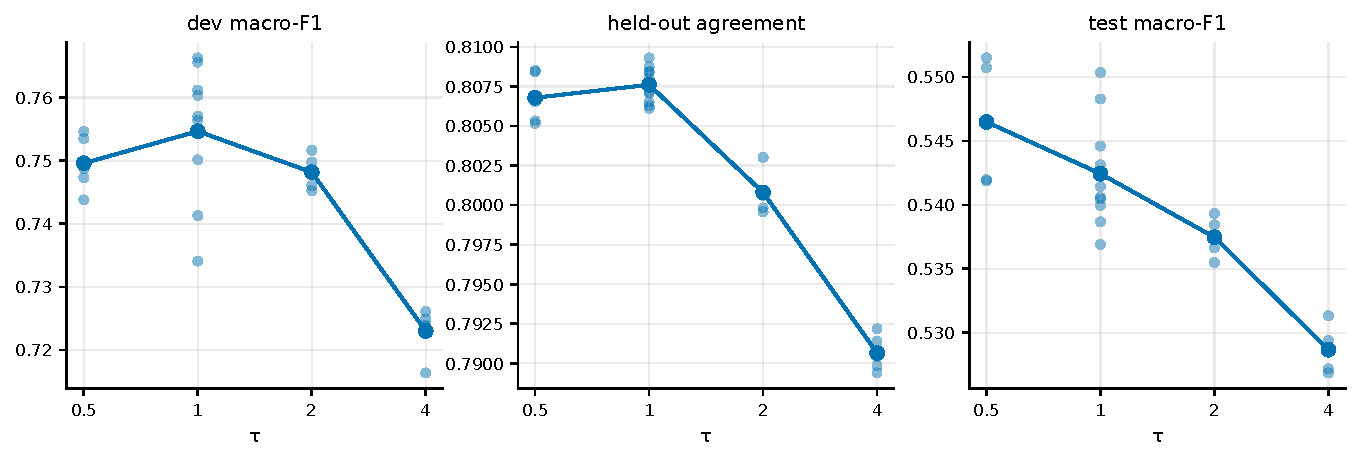
\includegraphics[width=0.9\textwidth]{figures/fig_temperature.pdf}
\caption{Effect of the distillation temperature. Each dot is one seed. The line connects the means.}
\label{fig:temperature}
\end{figure*}

\begin{figure}[!t]
\centering
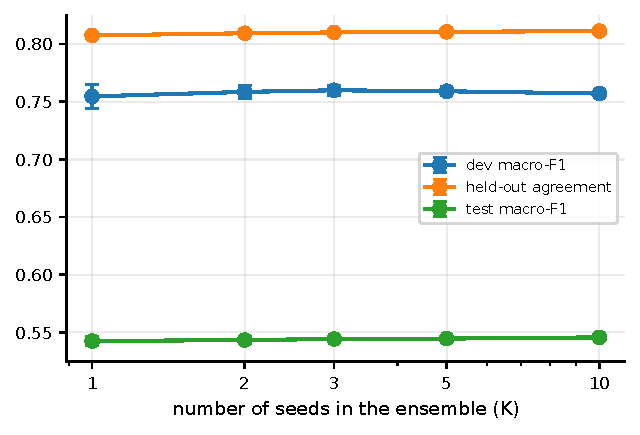
\includegraphics[width=0.85\columnwidth]{figures/fig_ensemble_size.pdf}
\caption{Effect of the table ensemble size (mean $\pm$ standard deviation over seed combinations).}
\label{fig:ensemble}
\end{figure}

\subsection{CPU Efficiency (RQ3)}
\label{sec:res-eff}
\begin{table*}[!t]
\caption{CPU Efficiency on Pinned P-Cores (Sample From the Unified Test Set, 1c/4c = 1/4 Cores)}
\label{tab:eff}
\centering
\footnotesize
\resizebox{\textwidth}{!}{%
\begin{tabular}{@{}lcccccl@{}}
\toprule
Model & Latency p50 / p95, 1c (ms) & Throughput 1c (doc/s) & Throughput 4c (doc/s) & Model RAM (MB) & File (MB) & Dependencies \\
\midrule
Teacher XLM-R-large & 2,971 / 3,210 & 0.33 & 0.76 & 2,957 & 2,136 & torch, transformers \\
Teacher XLM-R-large, ONNX int8 & 1,239 / 1,279 & 0.77 & 2.62 & 1,383 & 537 & onnxruntime, transformers \\
DistilmBERT + KD & 198 / 215 & 4.88 & 14.6 & 1,068 & 516 & onnxruntime, transformers \\
MiniLM-L6 + KD & 57.8 / 68.5 & 16.4 & 36.5 & 1,242 & 408 & onnxruntime, transformers \\
\textbf{StaticKD} & \textbf{2.03 / 3.46} & \textbf{473} & \textbf{893} & 501 & \textbf{34} & numpy, tokenizers \\
StaticKD-compact & 1.87 / 3.32 & 549 & 1,851 & 277 & 23 & numpy, tokenizers \\
fastText + KD, subword, quantized & 2.08 / 3.95 & 532 & 892 & 300 & 18 & fasttext, tokenizers \\
fastText + KD, subword & 2.26 / 4.30 & 455 & 592 & 1,121 & 839 & fasttext, tokenizers \\
TF-IDF + SVM + KD & 2.93 / 4.48 & 421 & 595 & 826 & 166 & scikit-learn, tokenizers \\
\bottomrule
\end{tabular}}
\end{table*}
On CPU, the teacher is too slow for a large stream of articles. StaticKD removes this cost almost entirely (Table~\ref{tab:eff}, Figs.~\ref{fig:tradeoff} and~\ref{fig:latency}). In PyTorch fp32, the teacher needs 2,971~ms per article on one core, with a throughput of 0.33 articles per second. The best CPU configuration for the teacher is ONNX int8, with 1,239~ms per article and a throughput of 0.77 articles per second. Classifying one million articles per day would take 15.1 cores (ONNX int8) to 34.8 cores (PyTorch) for this step alone.

StaticKD needs 2.03~ms per article and can process 473 articles per second per core. Its speed is about 616 times that of the ONNX int8 teacher and 1,420 times that of the PyTorch teacher. Compared with MiniLM-L6, StaticKD is about 29 times faster. Its file is 16 times smaller than that of the ONNX int8 teacher, and a load of one million articles per day needs 0.02 cores. The model uses 501~MB of RAM, mostly for the tokenizer structure, while the compact variant uses 277~MB. Tokenization takes 98\% of the single-thread prediction time and produces 579 tokens per article on average. Averaging the table rows alone runs at 28,755 articles per second. The speed of StaticKD is thus limited by the tokenizer, not by the model.

StaticKD is not the fastest model in the table. The quantized fastText + KD is slightly faster, at 532 articles per second. It is also smaller (18~MB) and uses less RAM (300~MB). Despite these three advantages, its test macro-F1 is 0.435, lower than the 0.545 reached by StaticKD. Four models have comparable latency: StaticKD, its compact variant, fastText, and TF-IDF + SVM. Among them, StaticKD is the most accurate, as shown in Fig.~\ref{fig:tradeoff}.

\begin{figure}[!t]
\centering
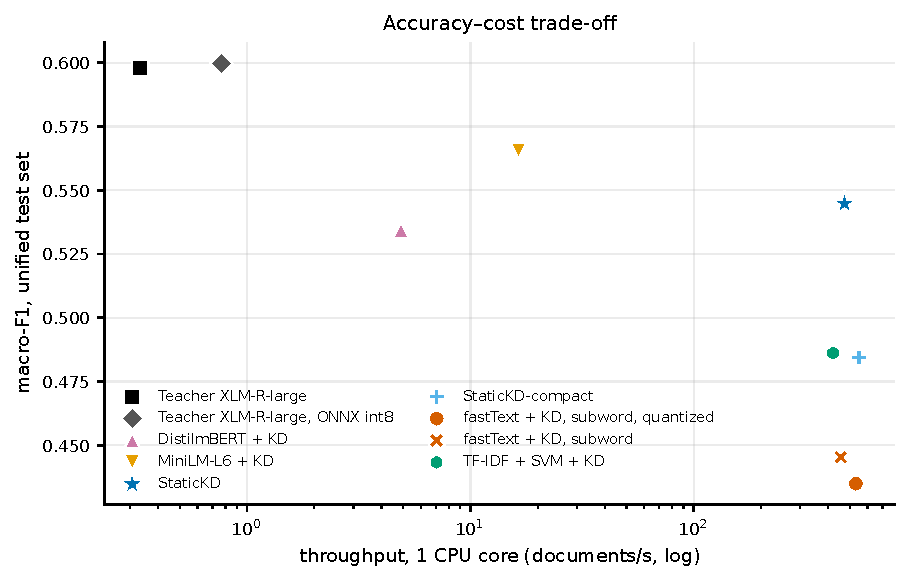
\includegraphics[width=\columnwidth]{figures/fig_tradeoff.pdf}
\caption{Test macro-F1 on the unified test set against single-core CPU throughput (log scale).}
\label{fig:tradeoff}
\end{figure}

\begin{figure*}[!t]
\centering
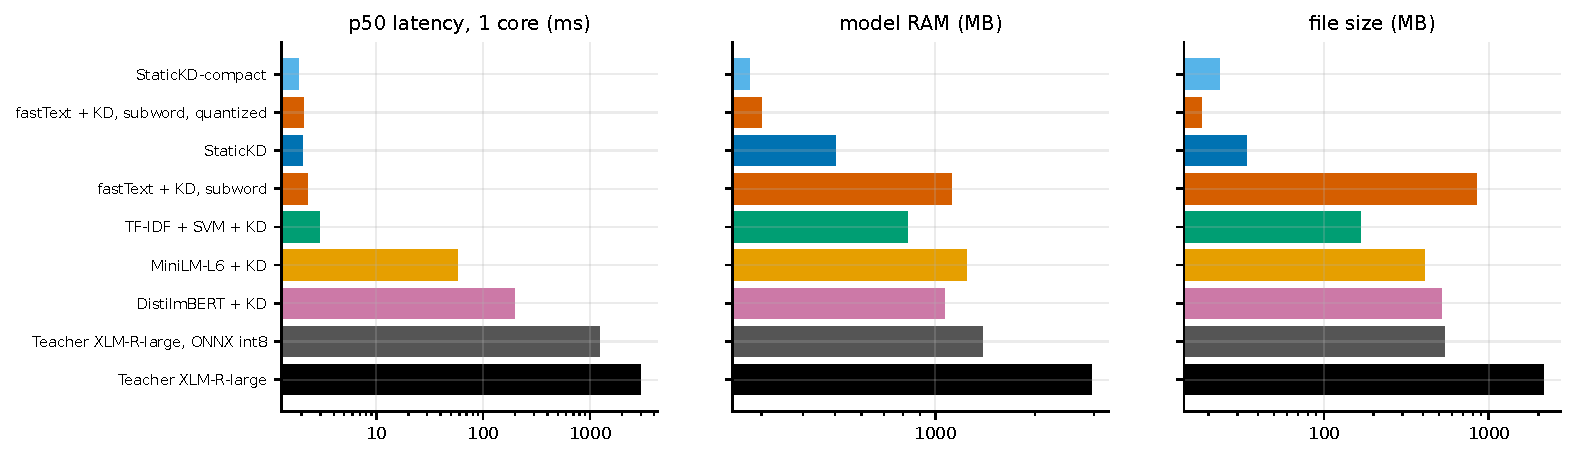
\includegraphics[width=0.9\textwidth]{figures/fig_latency_ram_size.pdf}
\caption{Latency per article, model RAM, and file size (log scale).}
\label{fig:latency}
\end{figure*}

\subsection{Analysis by Language and Label (RQ4)}
\label{sec:res-lang}
\begin{table}[!t]
\caption{Factors Behind Per-Language Performance}
\label{tab:factors}
\centering
\footnotesize
\setlength{\tabcolsep}{3pt}
\resizebox{\columnwidth}{!}{%
\begin{tabular}{@{}lcc@{}}
\toprule
Test & Statistic & $p$ \\
\midrule
Spearman: agreement vs log(distillation data) & $\rho=0.31$ & 0.022 \\
Spearman: agreement vs number of training sites & $\rho=0.29$ & 0.033 \\
Spearman: agreement vs teacher confidence & $\rho=0.71$ & $<$0.001 \\
Kruskal--Wallis: across scripts & $H=10.37$ & 0.065 \\
Spearman (test): accuracy gap vs log(data) & $\rho=0.52$ & $<$0.001 \\
Spearman (test): StaticKD accuracy vs token coverage & $\rho=0.50$ & $<$0.001 \\
Spearman (test): accuracy gap vs token coverage & $\rho=0.49$ & $<$0.001 \\
\bottomrule
\end{tabular}}
\end{table}
In a typical language, the accuracy of StaticKD is close to that of the teacher, with a median per-language accuracy gap of $-$0.024 (Fig.~\ref{fig:lang}). Table~\ref{tab:factors} relates this gap to properties of the language. The analysis on the held-out set uses 53 languages with at least 20 documents each. The agreement of StaticKD with the teacher rises with the log amount of distillation data ($\rho=0.31$, $p=0.022$) and with teacher confidence ($\rho=0.71$, $p<0.001$). The difference in agreement across scripts is not significant (Kruskal--Wallis $H=10.37$, $p=0.065$). The weak spot of StaticKD is a group of African languages. StaticKD reaches a mean accuracy of only 0.407 on languages that lie outside XLM-R pre-training and are also absent from the distillation data (ig, lg, ln, pcm, rn, sn, ti, yo). The teacher reaches 0.643 on the same languages.

Four Indian languages (bn, ml, or, pa) show how StaticKD behaves on text whose tokens hardly ever appeared in training. In these languages, at least 68\% of the token occurrences come from tokens that appear fewer than 10 times in the distillation data. StaticKD still reaches a mean accuracy of 0.624 there, against 0.738 for the teacher. The compact variant removes these rare tokens from the tokenizer, and its accuracy on these four languages falls to 0.013. In the other languages, the compact variant reaches an accuracy of 0.578, against 0.640 for the full StaticKD.

\begin{figure*}[!t]
\centering
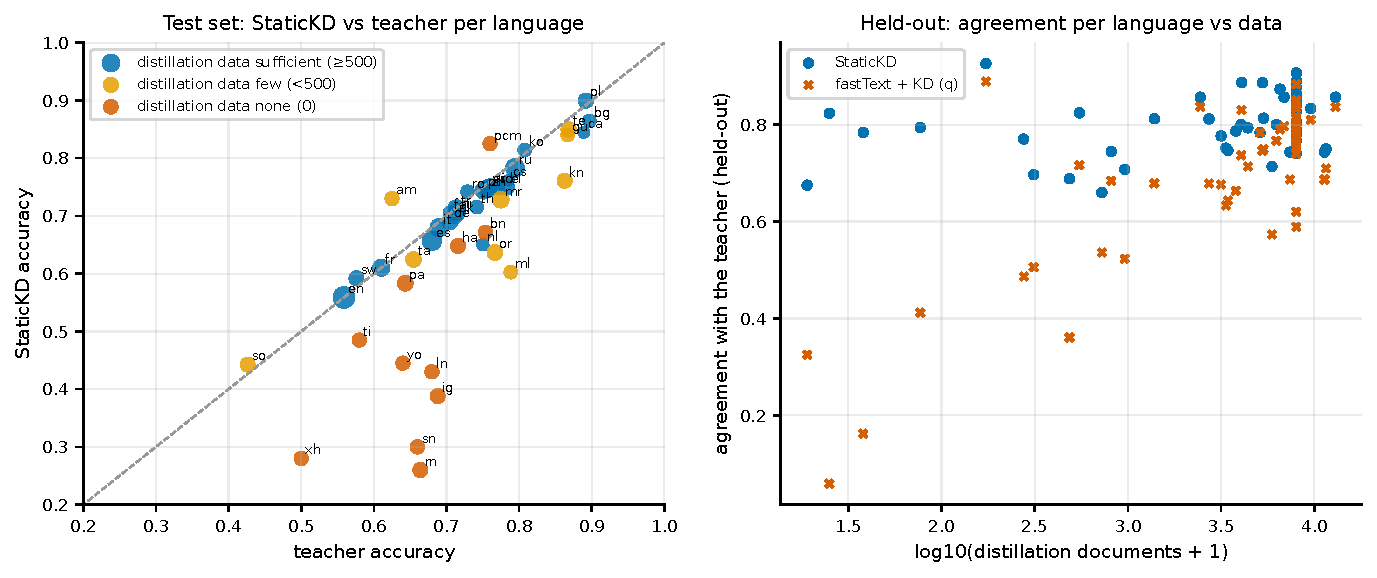
\includegraphics[width=0.9\textwidth]{figures/fig_per_language.pdf}
\caption{Left: StaticKD accuracy against teacher accuracy per test language (color shows the distillation data of the language, size the number of articles). Right: held-out agreement per language against the amount of distillation data for StaticKD and fastText + KD.}
\label{fig:lang}
\end{figure*}

Fig.~\ref{fig:label} shows the results per label. For StaticKD, the hardest labels are \emph{society} (0.16), \emph{disaster} (0.29), \emph{human interest} (0.32), and \emph{conflict} (0.37). The easiest labels are \emph{sport} (0.88), \emph{weather} (0.84), and \emph{education} (0.75). Against the teacher, the largest gaps occur for \emph{environment} ($-$0.17), \emph{religion} ($-$0.15), and \emph{arts} ($-$0.08). The most frequent confusions are \emph{society} $\rightarrow$ \emph{human interest}, \emph{human interest} $\rightarrow$ \emph{arts}, and \emph{society} $\rightarrow$ \emph{politics}, with 20\% each.

The table also shows which tokens carry the topic signal of an article. The specificity of a token is defined as the largest difference between one entry of its table row and the mean of the other 16 entries. Keeping only the 10\% most specific tokens of each article (about 58 tokens per article) leaves the test macro-F1 almost unchanged (0.543 against 0.545). In contrast, a random 10\% of the tokens gives 0.435.

\begin{figure*}[!t]
\centering
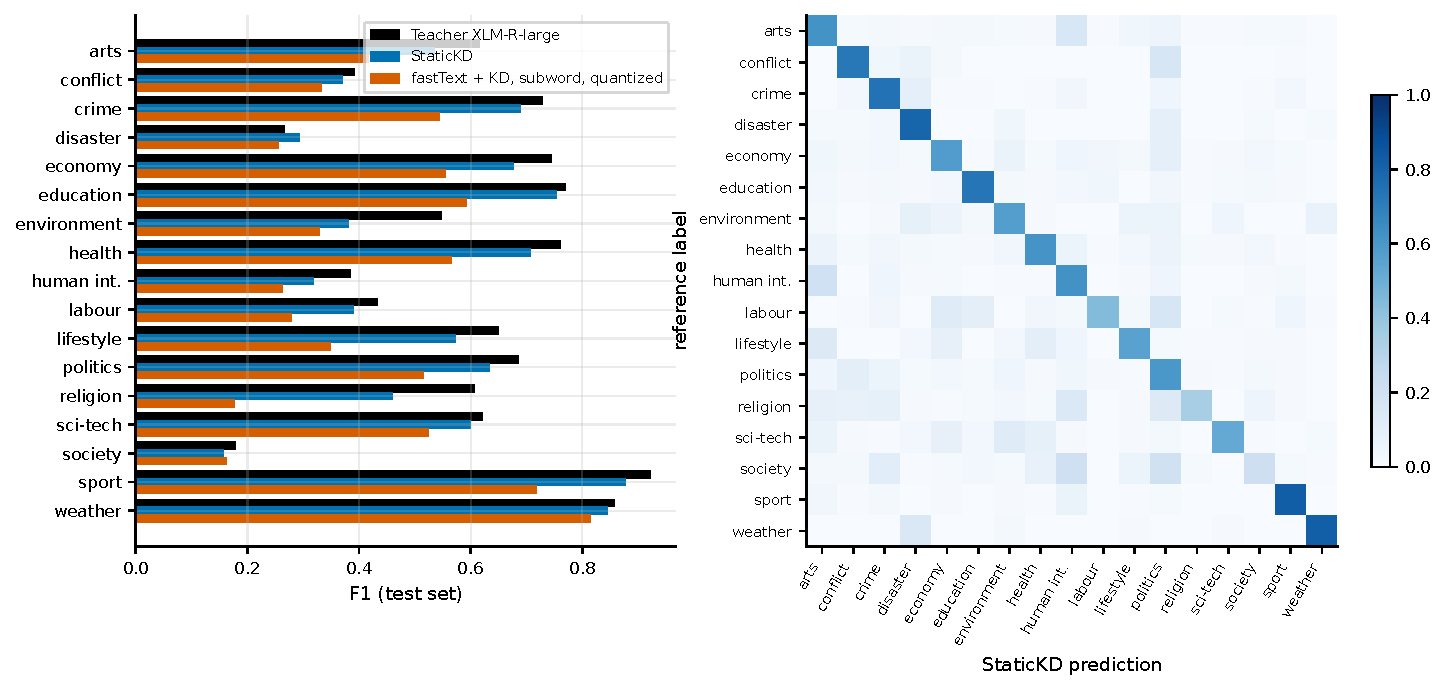
\includegraphics[width=0.9\textwidth]{figures/fig_per_label.pdf}
\caption{F1 per label on the test set (left) and the StaticKD confusion matrix normalized per reference label (right).}
\label{fig:label}
\end{figure*}

\subsection{Calibration and Cascade Mode}
\begin{table}[!t]
\caption{Cascade StaticKD $\rightarrow$ ONNX Int8 Teacher on the Test Set (Effective Single-Core Throughput)}
\label{tab:cascade}
\centering
\footnotesize
\setlength{\tabcolsep}{2.5pt}
\resizebox{\columnwidth}{!}{%
\begin{tabular}{@{}lccccc@{}}
\toprule
$\theta$ & StaticKD share & Accuracy on share & Macro-F1 & Accuracy & doc/s \\
\midrule
0 (StaticKD only) & 100.0\% & 0.641 & 0.545 & 0.641 & 473 \\
0.5 & 80.8\% & 0.732 & 0.586 & 0.690 & 3.97 \\
0.6 & 74.0\% & 0.760 & 0.593 & 0.697 & 2.93 \\
0.7 & 67.4\% & 0.788 & 0.600 & 0.702 & 2.34 \\
0.8 & 60.3\% & 0.813 & 0.602 & 0.703 & 1.92 \\
0.9 & 51.7\% & 0.839 & 0.602 & 0.703 & 1.58 \\
Teacher only & 0.0\% & -- & 0.600 & 0.699 & 0.77 \\
\bottomrule
\end{tabular}}
\end{table}
The ECE of StaticKD is lower than that of the teacher. It is 0.041 on the development set and 0.139 on the test set, against 0.090 and 0.245 for the teacher. The test set lies outside the training distribution, and both models become overconfident there (Fig.~\ref{fig:calib}). In the cascade mode reported in Table~\ref{tab:cascade}, StaticKD itself decides the articles on which its confidence is at least $\theta$ and passes the rest to the teacher. At $\theta=0.8$, StaticKD decides 60.3\% of the articles and classifies them with an accuracy of 0.813. The cascade reaches an overall accuracy of 0.703 and a macro-F1 of 0.602, compared with 0.699 and 0.600 for the teacher alone. Its effective throughput is 1.92 articles per second per core, against 0.77 for the teacher.

\begin{figure}[!t]
\centering
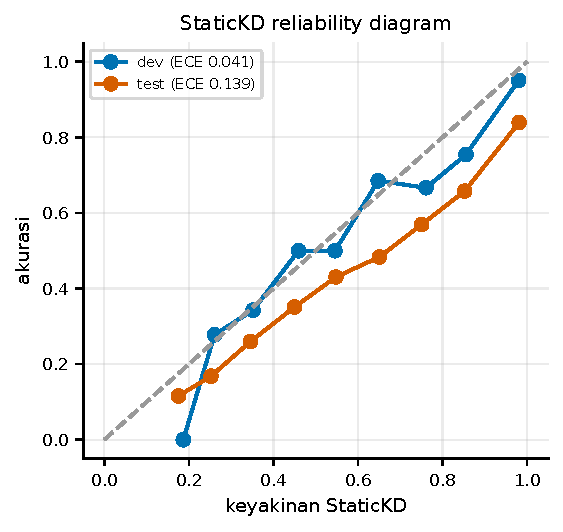
\includegraphics[width=0.8\columnwidth]{figures/fig_calibration.pdf}
\caption{Reliability diagram of StaticKD on the development and test sets.}
\label{fig:calib}
\end{figure}

\section{Discussion}
\label{sec:discussion}
The results in Sections~\ref{sec:res-acc} and~\ref{sec:res-eff} show that a table lookup keeps about nine tenths of the teacher macro-F1, while its inference cost is two to three orders of magnitude lower. This finding agrees with~\cite{galke2022bow}, which showed that order-free representations are already competitive for topic classification. The token analysis in Section~\ref{sec:res-lang} explains why a table suffices. Almost all of the topic signal in an article is carried by a small share of topic-specific tokens. The remaining gap to the teacher has two sources. The first source is a small number of labels on which StaticKD falls furthest behind the teacher, namely \emph{environment}, \emph{religion}, and \emph{arts} (Fig.~\ref{fig:label}). The lowest StaticKD scores are a separate matter. They occur on \emph{society}, \emph{disaster}, \emph{human interest}, and \emph{conflict}. The teacher also finds these labels among the hardest. Even for human annotators, \emph{society} and \emph{human interest} are known to be difficult~\cite{kuzman2025llm}. The low scores on these labels are therefore not specific to the student. The second source is languages that are underrepresented in the distillation data, as shown in Table~\ref{tab:groups}.

With the same distillation data, MiniLM-L6 closes part of this gap, whereas DistilmBERT does not (Table~\ref{tab:sig}). Both models cost one to two orders of magnitude more than StaticKD. The two models have different origins. MiniLM comes from a distillation of XLM-R-large, while DistilmBERT comes from mBERT. This difference suggests that the quality of the initial multilingual representation matters more than the number of layers.

For RQ2, the ablations show where the knowledge of the student comes from. The largest contribution comes from the pre-trained multilingual initialization. Without this initialization, the test macro-F1 drops by 0.120, whereas removing the multilingual data lowers it by 0.051. Next come the multilingual distillation data labeled by the teacher. This is consistent with Sparse Distillation~\cite{ye2022sparse}, which also relies on a large amount of teacher-labeled text. The most direct evidence for the role of the initialization comes from the compact variant. Some Indian languages hardly occur in the distillation data. Examples are bn, pa, and or (Odia). Most token occurrences in these languages come from tokens seen fewer than 10 times in the distillation data. The embeddings of these tokens are rarely or never updated, so they stay close to their potion values. The mean accuracy of StaticKD in these languages is still 0.624, but it falls to 0.013 once the compact tokenizer removes these tokens. Transfer to languages without data therefore relies on embeddings that training hardly changes. They lie in the same space as the trained embeddings, so the linear head learned from data-rich languages still applies to them.

The other side of the same mechanism appears in the frozen-embedding ablation. During fine-tuning, the embeddings of tokens from the training languages move, and the model fits these languages better. For this reason, frozen embeddings give a lower development score. Tokens from other languages stay at the positions that potion gave them. The head of the model has adapted to the moved embeddings, so these tokens fit it less well. This mechanism explains why frozen embeddings are better in languages with little or no distillation data. The final recipe still uses fine-tuning because it was selected on a development set in the training languages. Such a development set cannot reveal this effect. When a deployment targets languages without distillation data, the safer choice is frozen embeddings or a regularizer that keeps the embeddings close to potion. Both can still be folded into a table.

Soft labels, by contrast, add little or nothing. At $\tau=1$, hard teacher labels do not differ significantly from soft labels, and no higher temperature improves on $\tau=1$ (Section~\ref{sec:res-abl}). This pattern fits the literature on the capacity gap~\cite{zhang2025law,wang2026rckd}. A possible explanation is that one linear layer over averaged embeddings cannot represent the inter-class structure in the tail of the teacher distribution (dark knowledge)~\cite{zhao2022dkd}. An attainable target for the student comes from a sharp distribution ($\tau=1$) or from hard labels. With a high $\tau$, the student is asked to imitate a distribution shape beyond its capacity. For very-low-capacity students, effort is more useful when spent on the coverage of the distillation data (languages, sites, topics) and on a multilingual initialization, not on shaping the soft labels.

Per-language performance is determined mainly by how well a language is represented in the distillation data and the pre-training data. The script is not the determining factor (Kruskal--Wallis $p=0.065$). The weakest results appear in African languages outside XLM-R pre-training that are also absent from the distillation data: ig, lg, ln, pcm, rn, sn, ti, and yo. The teacher still reaches an accuracy of 0.643 on these languages, perhaps thanks to subwords shared with other languages and to sentence context. StaticKD reaches only 0.407. The cheapest fix requires no change of architecture. News in these languages can simply be added to the distillation data and then labeled by the teacher. This step is supported by the data ablation and by the correlation between agreement and the amount of data ($\rho=0.31$).

Agreement with the teacher cannot always be used to predict accuracy on editorial labels. The frozen-embedding variant scores 0.020 lower in held-out agreement but 0.014 higher in test macro-F1. Cutting the data to 130 thousand documents lowers the agreement ($-$0.009) without a significant change on the test set ($-$0.002). Student selection should not rely on agreement with the teacher alone. In line with~\cite{stanton2021kd}, it should use labels that do not come from the teacher and a development set outside the training distribution.

Test scores should be read with the nature of the labels in mind. For example, an article about a criminal case that involves an athlete can rightly sit in a sports section, while a model labels it \emph{crime}. IPTC allows several topics per article, so both answers are plausible. Comparisons between models remain fair because all models are scored against the same labels. The model ranking also does not change on the subset in which the number of articles per site is capped.

Sparse Distillation~\cite{ye2022sparse} uses an n-gram table trained from scratch. StaticKD replaces it with pre-trained multilingual embeddings folded into 17 logits per token. With this replacement, the model becomes far smaller and can transfer to languages that are missing from the distillation data. In a news pipeline, inference is a recurring cost because every incoming article has to be classified. For one million articles per day, the ONNX int8 teacher needs 15.1 cores, whereas StaticKD needs only 0.02 cores (Section~\ref{sec:res-eff}).

In a real-time pipeline on servers without a GPU, StaticKD needs a 34~MB file, and its only dependencies are \texttt{numpy} and \texttt{tokenizers}. Its output probabilities are better calibrated than those of the teacher, with a test ECE of 0.139 against 0.245. The better calibration makes a cascade mode possible. At $\theta=0.8$, the cascade accuracy of 0.703 is on par with that of the teacher alone (0.699). The cascade throughput is 1.92 articles per second per core, against 0.77 for the teacher alone. This mode suits batch jobs that need teacher-level accuracy. The compact variant lowers RAM, but it is only advisable when all target languages are already covered by the distillation data.

\section{Limitations}
\label{sec:limitations}
Of the test articles, 47.5\% carry section labels from JSON-LD, and 20.4\% carry publisher categories. Section conventions differ from one publisher to another. A section also reflects one editorial view of an article that may cover several topics at once. The mapping table was built conservatively, validated against the IPTC tree, and reviewed by the first author. However, the articles were not re-annotated by humans. Absolute scores on these labels therefore measure agreement with the way publishers categorize articles. This holds especially for labels with unclear boundaries, such as \emph{society}, \emph{human interest}, and \emph{lifestyle}.

In MasakhaNEWS, labels were assigned by human annotators under their own scheme and then mapped to IPTC. Direct annotation with IPTC topics exists only in MN-DS, which is entirely in English. Kuzman and Ljube\v{s}i\'c~\cite{kuzman2025llm} have a multilingual IPTC test set, but it is not public, so it was not available for this study.

The number of labels that occur in each language is uneven. The median is 7 labels per language, and the African languages cover only four or five broad topics. Because macro-F1 is computed over the labels present, per-language scores cannot be compared directly between languages with different label coverage. Publisher diversity is also limited. Twenty-seven languages come from practically one publisher: BBC/VOA for the African languages, L3Cube for the Indian languages, and a single site for several CC-NEWS languages. Claims about these languages hold only for those publishers. The site-cluster bootstrap widens their confidence intervals accordingly.

The teacher bounds the performance of the student from above. Its errors and biases are also copied to the student. The held-out set measures agreement with the teacher, not correctness.

The tuning budget was not equal across models. The StaticKD recipe was selected from 72 runs on the development set, whereas the hyperparameters of fastText and TF-IDF + SVM were set once without a search. This imbalance may widen the accuracy gap to these two baselines. Two related methods were not run as baselines. The first is Sparse Distillation~\cite{ye2022sparse}. It differs from fastText + KD and from the random-initialization ablation in the hidden layers of its deep averaging network, its soft-logit targets, and its billion-parameter n-gram table designed for English. The second is the classifier trainer of Model2Vec~\cite{tulkens2024model2vec}. It trains on hard labels, adds a 512-unit hidden layer, and learns a weight for each token. The ablations test hard labels and a 512-unit hidden layer separately. Neither differs significantly from the final recipe on the development set or on the test set (Table~\ref{tab:ablation}). Their combination has not been tested, and neither have the learned token weights. A model with a hidden layer also cannot be folded into one table. MiniLM-L6 and DistilmBERT were trained and evaluated with inputs of at most 256 tokens. As a result, both models see less than half of the text of most test articles, so their accuracy may be underestimated.

The whole benchmark ran on one machine in one session. For the teacher and the transformers, latency was measured on 30 documents. Absolute numbers on a server will differ, and the latency sample for these heavy models is small. Even so, ratios between models measured under the same protocol remain informative.

StaticKD is much less accurate on African languages that are absent from both the distillation data and the pre-training data (Section~\ref{sec:discussion}). If this model is used as a topic filter, news in these languages could be misclassified or dropped more often. During deployment, accuracy should be monitored per language. Articles with low confidence should be routed to the teacher through the cascade mode.

The scope of this study is limited to top-level IPTC labels and single-label classification. Labels at deeper levels and multi-topic articles have not been tested.

\section{Conclusion}
\label{sec:conclusion}
On one CPU core, the open multilingual IPTC classifier needs 1.2 to 3 seconds per article. StaticKD distills this classifier into a table of 17 logits per token. The table is initialized from multilingual static embeddings and then trained on 285,999 teacher-labeled articles in 69 languages. The evaluation uses 12,744 test articles in 47 languages, with labels that do not come from the teacher. On this set, StaticKD reaches a macro-F1 of 0.545, or 91.1\% of the teacher score. It processes 473 articles per second per CPU core, about 616 times the speed of the ONNX int8 teacher. This 34~MB model also needs no deep learning library.

The accuracy of this very small student has two main sources: multilingual distillation data and pre-trained multilingual embeddings. Soft labels are no better than hard labels. Fine-tuning the embeddings raises accuracy in the training languages but lowers it in languages without distillation data, i.e., languages whose embeddings are rarely or never updated during training. StaticKD is weakest on languages that appear in neither the distillation data nor the pre-training data of the teacher. Its hardest labels are \emph{society}, \emph{disaster}, \emph{human interest}, and \emph{conflict}. The test set of this study can be reused to evaluate other IPTC classifiers.

These results point to several directions for further research. The distillation data should be extended to the weak languages, especially the African languages outside XLM-R pre-training. Fine-tuning could also use a regularizer that keeps the embeddings close to the pre-trained space. Such a regularizer might give in-distribution accuracy and cross-lingual transfer at the same time. On the speed side, tokenization takes 98\% of the inference time. The next source of speed is therefore a faster tokenizer, for example, a direct word-to-table lookup. Any form of vocabulary pruning has to keep cross-lingual tokens. Several problems remain open: cheap non-linear heads with quantized embeddings, hierarchical classification down to IPTC level 2, multi-label classification, and human IPTC annotation of a multilingual sample of the test set.

\section*{Code, Model, and Data Availability}
The code for this study is available at \todo{GitHub URL and Zenodo DOI}. It covers data collection, test-set construction, teacher labeling, training, evaluation, and benchmarking. The same location provides a notebook that reproduces every number, table, and figure in this paper. The section-to-IPTC mapping table is also released with the code. The StaticKD models are available at \todo{Hugging Face URL}. The test set is released as a manifest of article URLs or IDs, labels, label origins, and text hashes, together with a reconstruction script. The article texts themselves are not redistributed because of publisher copyright and the licenses of the source datasets. EMMediaTopic is available from the CLARIN.SI repository~\cite{emmediatopic2025}. Table~\ref{tab:license} lists the licenses of the assets used and released in this study.

\begin{table}[!t]
\caption{Licenses of the Assets Used and Released}
\label{tab:license}
\centering
\footnotesize
\setlength{\tabcolsep}{3pt}
\resizebox{\columnwidth}{!}{%
\begin{tabular}{@{}ll@{}}
\toprule
Asset & License \\
\midrule
Teacher \texttt{classla/multilingual-IPTC-news-topic-classifier} & CC BY-SA 4.0 \\
Embeddings \texttt{minishlab/potion-multilingual-128M} & MIT \\
MasakhaNEWS & CC BY-NC 4.0 \\
MN-DS, L3Cube-IndicNews, IndoNews & CC BY 4.0 \\
Bangla news~\cite{hossain2025banglanews} & not stated on the dataset card \\
EMMediaTopic 1.0 & CC BY-SA 4.0 \\
CC-News 2019--2021, CC-NEWS 2024--2026 & Common Crawl terms of use \\
\midrule
StaticKD code (release) & MIT \\
StaticKD models (release) & CC BY-SA 4.0 (inherited from the teacher) \\
Test-set manifest (release) & CC BY-SA 4.0 \\
\bottomrule
\end{tabular}}
\end{table}

\section*{Acknowledgment}
The authors thank the Department of Informatics Engineering, Sepuluh Nopember Institute of Technology, for supporting this research. The authors used Claude Opus 5.5 (Anthropic) to assist with writing the experiment code, with data processing (including the first draft of the section-to-IPTC mapping table, all of which the authors reviewed), and with reviewing and minor editing of the manuscript. The manuscript was written by the authors, who take full responsibility for its content and claims.

\bibliographystyle{IEEEtran}
\bibliography{references}

\end{document}